%
% Portuguese-BR vertion
% 
\documentclass{report}

\usepackage{ipprocess}
% Use longtable if you want big tables to split over multiple pages.
\usepackage{longtable}
\usepackage{tikz}
\usepackage[utf8]{inputenc} 
\usepackage[portuguese]{babel} % Uncomment for portuguese
\usepackage{siunitx
\usepackage{pdflscape}
\usepackage{verbatim}

\newcommand{\tab}[1]{\hspace{.2\textwidth}\rlap{#1}}


\sloppy

\graphicspath{{./pictures/}} % Pictures dir
\makeindex
\begin{document}

\DocumentTitle{Documento de Arquitetura}
\Project{\si\micro Risc}
\Organization{}
\Version{Build 1.0}

\capa
\newpage
\newpage

%%%%%%%%%%%%%%%%%%%%%%%%%%%%%%%%%%%%%%%%%%%%%%%%%%
%% Revision History
%%%%%%%%%%%%%%%%%%%%%%%%%%%%%%%%%%%%%%%%%%%%%%%%%%
\section*{\center Histórico de Revisões}
\begin{center}
\begin{longtable}[pos]{|m{50pt} | m{200pt} | m{100pt}|} \hline
	\cellcolor[gray]{0.9} \textbf{Data} & \cellcolor[gray]{0.9}\textbf{Descrição} & \cellcolor[gray]{0.9}\textbf{Autor(s)}\\ \hline \endfirsthead \hline
	\multicolumn{2}{|c|}{{\bfseries \textbf{continuação da tabela anterior}}} \\ \hline
	\textbf{Data} & \cellcolor[gray]{0.9}\textbf{Descrição} & \cellcolor[gray]{0.9}\textbf{Autor(s)}\\ \hline
	\multicolumn{2}{|c|}{{\textbf{continua na próxima página}}} \\ \hline \endfoot
	\hline \endlastfoot
	
  14/12/2015 &  Estruturação do documento &  Patricia Gomes\\ \hline  
  19/12/2015 &  Adição dos datapath's por instrução &  Fábio Barros\\ \hline 
  19/12/2015 &  Correção das tabelas &  Matheus Borges\\ \hline 
  19/12/2015 &  Criação do capítulo Assembly & Matheus Borges\\ \hline 
  19/12/2015 &  Criação das tabelas de entrada e saída dos módulos &  Patricia Gomes\\ \hline 
  19/12/2015 &  Preenchimento da tabela Acrônimos e Abreviações &  Matheus Borges\\ \hline
  19/12/2015 &  Preenchimento da tabela da tabela de sinais da unidade de controle &  Fábio Barros\\ \hline 
  19/12/2015 &  Criação do capítulo Requisitos do Processador  & Patricia Gomes \\ \hline 
  20/12/2015 &  Finalização do documento & Fábio Barros, Matheus Borges e Patricia Gomes\\ \hline
  20/12/2015 &  Revisão do documento & Fábio Barros e Matheus Borges \\ \hline
  15/01/2016 &  Alterações no documento & Patricia Gomes \\ \hline 
  20/01/2016 &  Correções do documento & Patricia Gomes \\ \hline 
  

\end{longtable}
\end{center}
\newpage
\tableofcontents
\newpage
\section{Introdução}
\subsection{Objetivo} 
O processador pode ser definido como o cérebro do computador, é ele o responsável por realizar todas as instruções dentro do computador como operações de lógicas e cálculos. Além disso ele é responsável pela tomada de decisões do sistema.

O objetivo deste documento de arquitetura é definir as especificações do processador desenvolvido. O documento de arquitetura é importante por permitir que outras pessoas possam utilizá-lo para construir um sistema a partir dele com sucesso. O mesmo  define os parâmetros de implementação que compõem os requisitos do processador implementado, tais requisitos incluem a arquitetura do conjunto de instruções, definições de entrada e saída e a arquitetura geral do processador. 

\subsection{Organização do Documento} 
\textbf{Sessão 2:} Apresenta uma visão geral da arquitetura e dos principais requisitos. \newline
\textbf{Sessão 3:} Especifica o conjunto de instruções do processador. \newline
\textbf{Sessão 4:} Especifica os elementos que compõem o sistema.\newline
\textbf{Sessão 5:} Descreve o montador. \newline

% inicio da tabela de acronimos e abreviacoes do documento
\subsection{Acrônimos e Abreviações}

\begin{center}
\begin{longtable}[pos]{|m{52pt} | m{350pt}|} \hline
	\cellcolor[gray]{0.9} \textbf{Sigla} & \cellcolor[gray]{0.9}\textbf{Descrição}\\ \hline \endfirsthead \hline
	\multicolumn{2}{|c|}{{\bfseries \textbf{continuação da tabela anterior}}} \\ \hline
	\cellcolor[gray]{0.9} \textbf{Sigla} & \cellcolor[gray]{0.9}\textbf{Descrição}\\ \hline \endhead
	\multicolumn{2}{|c|}{{\textbf{continua na próxima página}}} \\ \hline \endfoot
	\hline \endlastfoot
	
	GPR     & Registrador de Propósito Geral\\ \hline
    ISA     & Instruction Set Architecture - Conjunto de Instruções da Arquitetura\\ \hline
    IF      & Instruction Fetch - Busca da Instrução  \\ \hline
    ID      & Instruction Decode - Decoficação da Instrução \\ \hline
    RF      & Register Fetch -  Acesso aos Registradores\\ \hline
    EX      & Execute - Execução da Instrução\\ \hline
    MEM     & Memory - Acesso à Memória\\ \hline
    WB      & Write Back - Escrita de volta\\ \hline
    OP      & Operation Code - Código da Operação\\ \hline
    RA      & Read A - Ler A\\ \hline
    RB      & Read B - Ler B\\ \hline
    WC      & Write C - Escreve C\\ \hline
    CONTROL & Unidade de Controle\\ \hline
    COND    & Condição\\ \hline
    Const16 & Constante de 16 bits \\ \hline
    MI     & Memory Instruction (Memória de Instruções)\\ \hline
	PC     & Program Counter (Contador de Programa)\\ \hline
	RB     & Banco de Registradores\\ \hline
	UC     & Unit Control (Unidade de Controle)\\ \hline
	ALU    & Arithmetic Logic Unit (Unidade Lógica Aritmética)\\ \hline
	RF     & Register Flag (Registrador de Flags)\\ \hline
	TF     & Tests Flag (Testador de Flags)\\ \hline
	MX     & Multiplexer (Multiplexador)\\ \hline
	DM     & Data Memory (Memória de Dados)\\ \hline
	SE     & Signal Extender (Extensor de Sinal)\\ \hline
	RISC   & Reduced Instruction Set Computer (Computador com um Conjunto Reduzido de Instruções)\\ \hline

\caption{Tabela de acrônimos e abreviações}
\end{longtable}
\end{center}

\begin{comment}
\section{Requisitos do Processador}
É requerido que o processador desenvolvido seja capaz de executar instruções que possibilitem gerenciar a máquina de forma extremamente rápida e eficiente.\newline

A estrutura dos requisitos funcionais e não funcionais é descrita ao longo deste documento. Sendo requisito funcional e não funcional definidos na tabela abaixo:

% inicio da tabela
\FloatBarrier
\begin{table}[H]
    \begin{center}
        \begin{tabular}[pos]{|>{\arraybackslash}m{100pt}|>{\arraybackslash}m{290pt}|} 
          \hline
          \cellcolor[gray]{0.9}\textbf{Termos} & \cellcolor[gray]{0.9}\textbf{Descrição} \\ \hline
            Requisito Funcional   & Requisitos de hardware que compõem os módulos, descrevendo as ações que o mesmo deve estar apto a executar. \\ \hline
            Requisito Não Funcional   & Requisitos de hardware que compõem os módulos, representando as características que o mesmo deve ter, ou restrições que  o mesmo deve operar. \\ \hline
        \end{tabular}
        \caption{Tabela de Definição}
    \end{center}
\end{table}  

Os requisitos funcionais e não-funcionais são listados nas tabelas abaixo respectivamente:

% inicio da tabela
\FloatBarrier
\begin{table}[H]
    \begin{center}
        \begin{tabular}[pos]{|>{\arraybackslash}m{100pt}|>{\arraybackslash}m{290pt}|} 
          \hline
          \cellcolor[gray]{0.9}\textbf{Requisitos Funcionais} & \cellcolor[gray]{0.9}\textbf{Descrição} \\ \hline
           ISA composta por 42 instruções.  &  O processador deve ser capaz de executar 42 instruções.  \\ \hline
        \end{tabular}
        \caption{Tabela de Requisitos Funcionais}
    \end{center}
\end{table}  

% inicio da tabela
\FloatBarrier
\begin{table}[H]
    \begin{center}
        \begin{tabular}[pos]{|>{\arraybackslash}m{100pt}|>{\arraybackslash}m{290pt}|} 
          \hline
          \cellcolor[gray]{0.9}\textbf{Requisitos Não-Funcionais} & \cellcolor[gray]{0.9}\textbf{Descrição} \\ \hline
           Possuir 16 GPR de 32 bits de largura   & O processador deve possuir 15 registradores de propósito geral, sendo que cada registrador deve ser capaz de armazenar uma palavra de 32 bits. \\ \hline
           Arquitetura de 32 bits   & O processador deve suportar operações com operandos que possuam 32 bits. \\ \hline
        \end{tabular}
        \caption{Tabela de Requisitos Não-Funcionais}
    \end{center}
\end{table}  

Os requisitos foram atendidos, de forma que as instruções, apresentadas nas sessões seguintes, foram sugeridas a partir dos documentos de testes que foi entregue pelos solicitantes. A operação que cada instrução realiza é descrita em tabelas ao lado da intrução. 
\end{comment}
\newpage
\section{Visão Geral da Arquitetura}
Este documento descreve um processador µRISC adaptado à 32 bits. Esse processador possui 16 registradores de proposito geral e composta por um conjunto de 42 instruções. \newline
Para uma instrução ser executada são necessários quatro ciclos. Esses ciclos são denominados IF, ID, EX/MEN e WB, como apresentado na figura abaixo. No primeiro ciclo (IF),  a próxima instrução a ser executada, definida pelo contador de programa (PC), é lida da memória de instruções (MI). No segundo ciclo (ID), a instrução é identificada e os operandos são lidos do banco de registradores ou, em caso de operações com constantes, manipulado pelo extensor de sinal (SE). No terceiro ciclo (EX/MEM), a instrução é executa pela unidade lógica aritmética (ALU) ou pela memória, em caso de operações de armazenamento ou leitura. No quarto ciclo (WB), os resultados são escritos no banco de registradores.

\begin{figure}[H]
\centering
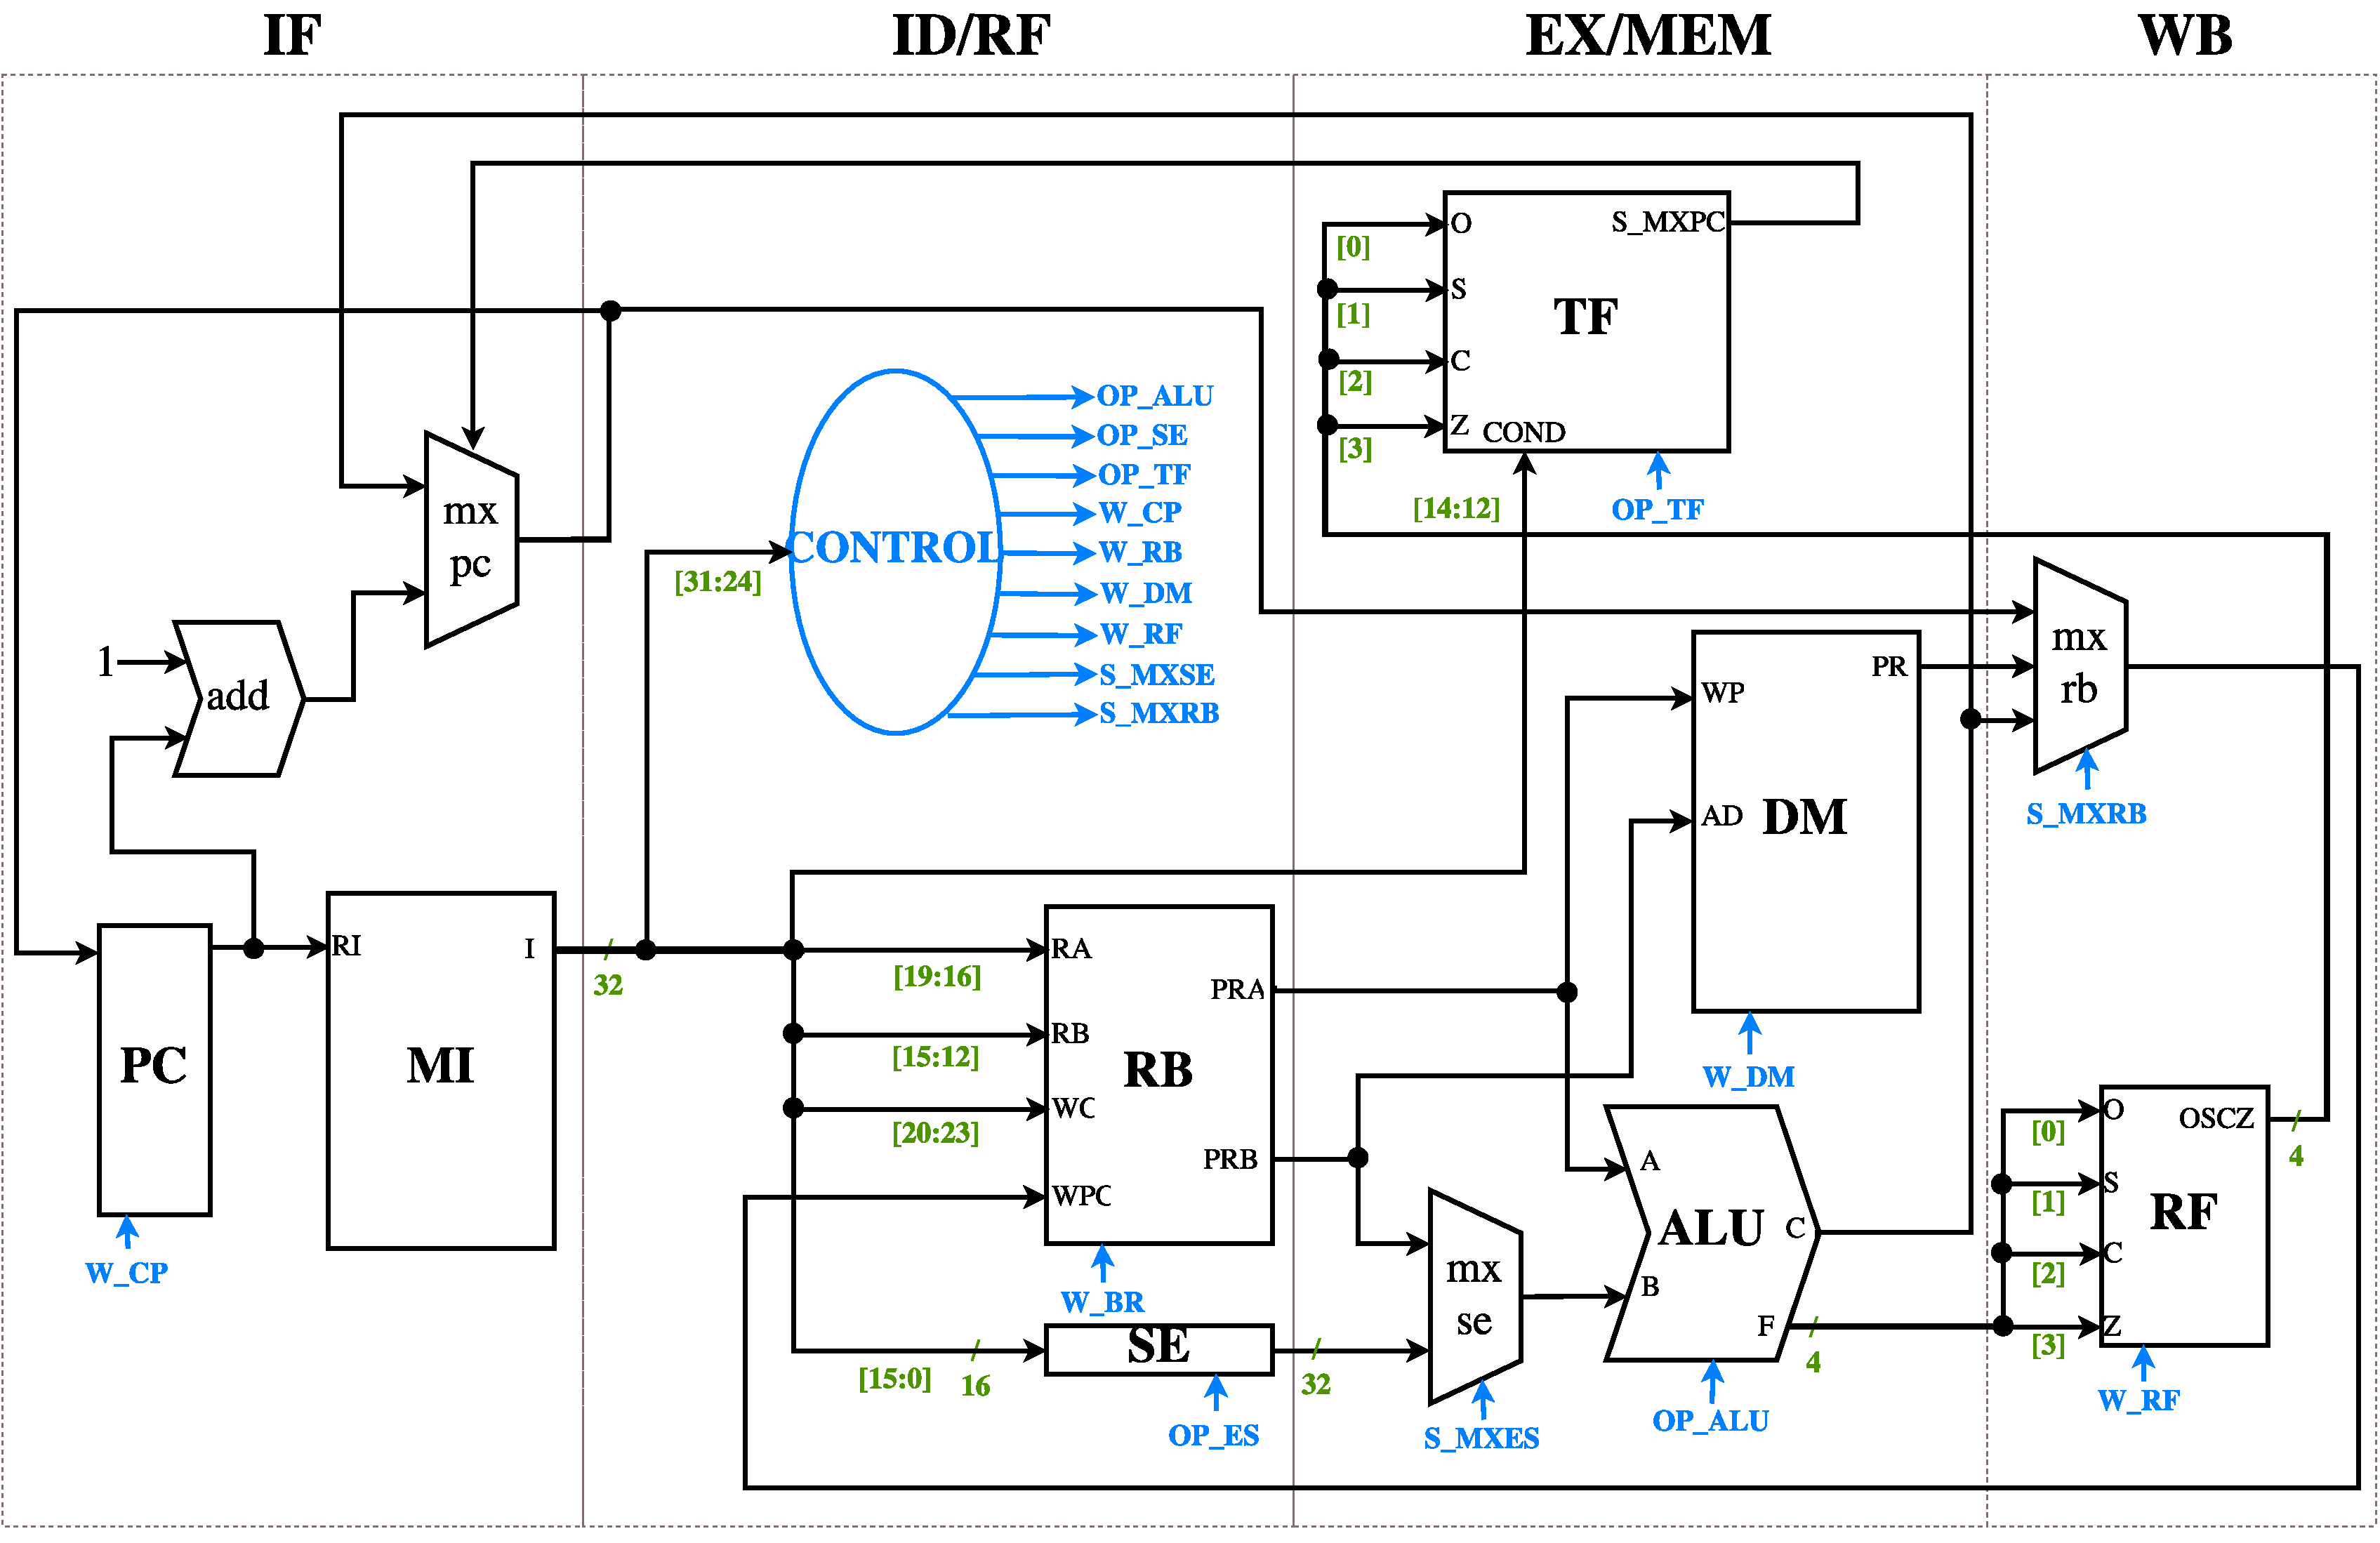
\includegraphics[width=\textwidth]{./pictures/Datapath.pdf}
\caption{Datapath Geral}
\end{figure}

\subsection{Principais características}
\begin{itemize}
    \item \textbf {Arquitetura de 32 bits;}
    \item \textbf {16 GPR de 32 bits de largura (r0 ... r15);}
    \item \textbf {ISA composta por 42 instruções;}
    \item \textbf {Instruções de até 3 operandos;}
    \item \textbf {Simulador e Montador desenvolvido na linguagem C;}
    \item \textbf {Armazenamento em memória de forma big-endian;}
    \item \textbf {Unidade de controle hardwired;}
    \item \textbf {Endereçamento por registrador e imediato;}
\end{itemize}

\newpage
\section{Arquitetura das Instruções}
O conjunto de instruções do processador foi dividido nos seguintes grupos:\newline
\begin{itemize}
    \item \textbf {Instruções lógicas e aritméticas;}
    \item \textbf {Instruções com constante;}
    \item \textbf {Instruções de acesso à memória;}
    \item \textbf {Instruções de desvio;}
    \item \textbf {Instruções de desvio por registrador;}
    \item \textbf {NOP;}
    \item \textbf {HALT;}
\end{itemize}

\subsection{Instruções Lógicas e Aritméticas}
\begin{figure}[H]
\centering
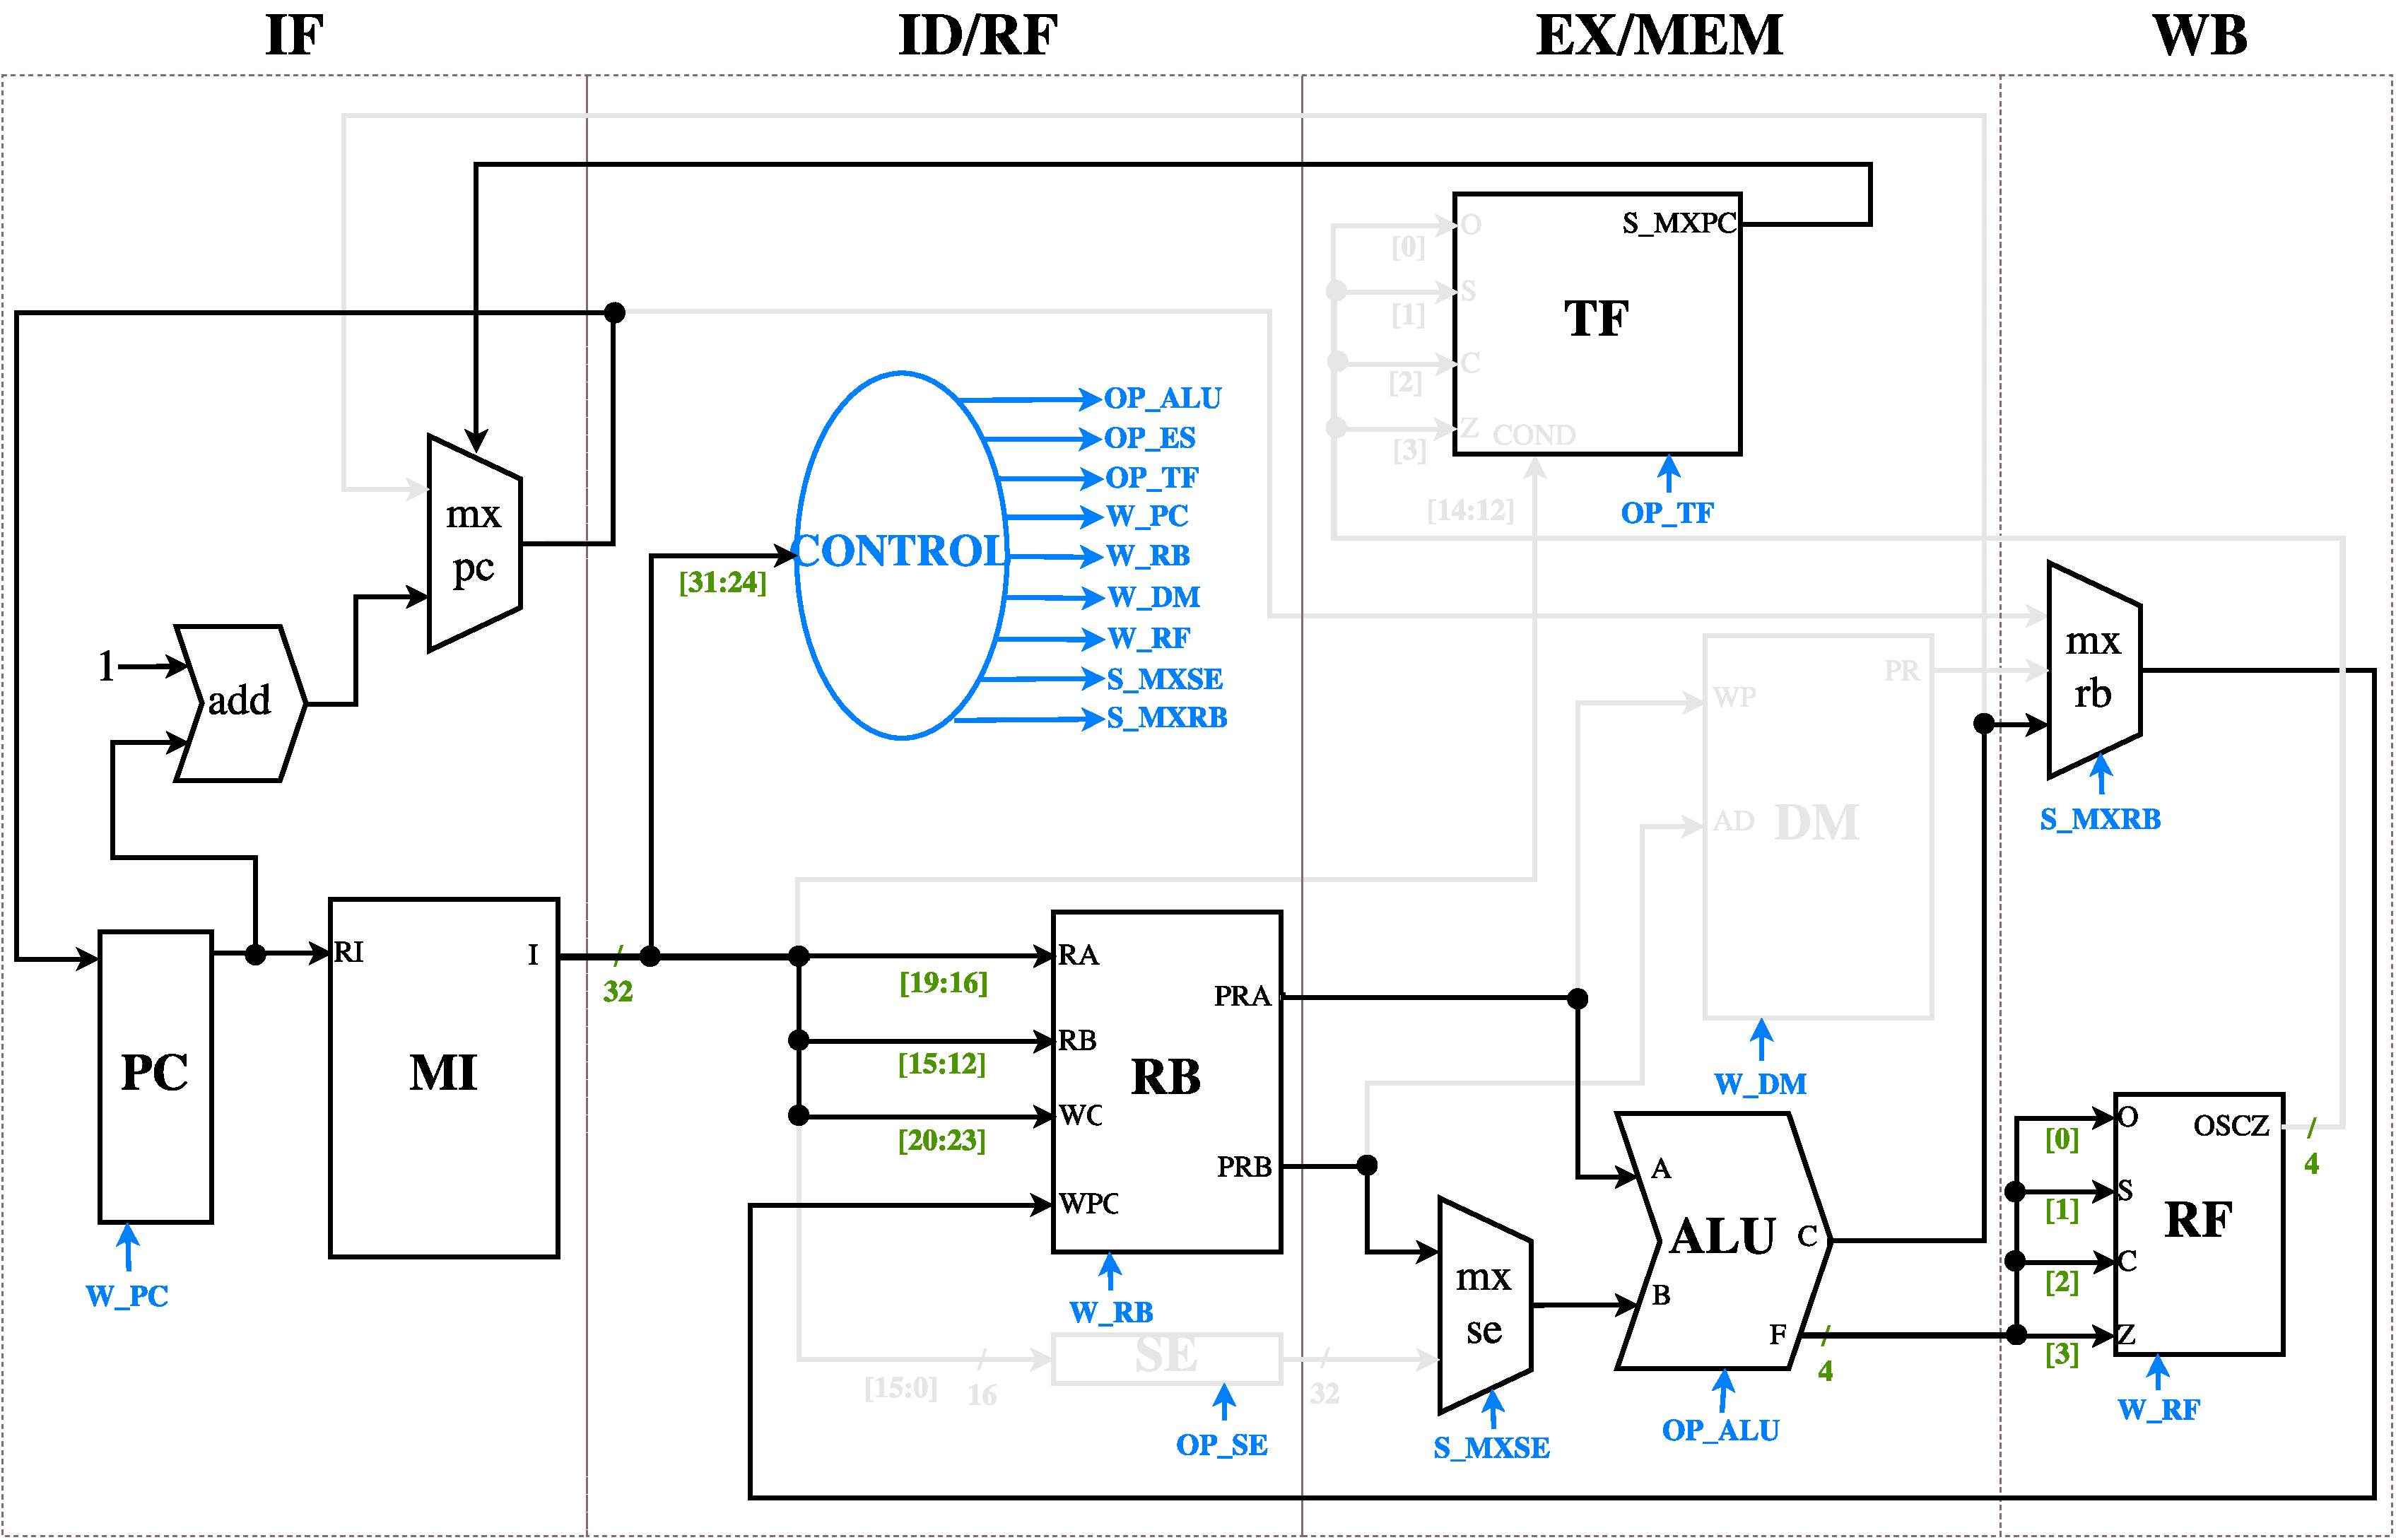
\includegraphics[width=\textwidth]{./pictures/DatapathLA.pdf}
\caption{Datapath de Lógicas Aritméticas}
\end{figure}


A Figura 2 apresenta o caminho de dados específico de instruções lógicas e aritméticas, nela é possível observar quais elementos participam da realização destas operações.\newline

Os elementos que caracterizam esse tipo de instrução são: 
\begin{itemize}
    \item Unidade logica aritmética (ALU): responsável por realiza a operação e gerar os sinais de flags;
    \item Registradores de flags (RF): responsável por armazena o último estado das flags atualizadas;
\end{itemize}
 

As instruções de lógica e aritmética possuem o seguinte formato:
% inicio da tabela de formato de instruções de lógica e aritmética
\FloatBarrier
\begin{table}[H]
    \begin{center}
    \renewcommand{\arraystretch}{1.5}
        \begin{tabular}[pos]{|>{\centering\arraybackslash}m{33pt}|>{\centering\arraybackslash}m{55pt}|>{\centering\arraybackslash}m{44pt}|>{\centering\arraybackslash}m{44pt}|>{\centering\arraybackslash}m{44pt}|>{\centering\arraybackslash}m{132pt}|} 
          \hline
          \cellcolor[gray]{0.9}\textbf{31:29} & \cellcolor[gray]{0.9}\textbf{28:24} & \cellcolor[gray]{0.9}\textbf{23:20} & \cellcolor[gray]{0.9}\textbf{19:16} & \cellcolor[gray]{0.9}\textbf{15:12} & \cellcolor[gray]{0.9}\textbf{11:0} \\ \hline
            0 0 1   & OP    & WC    & RA    & RB    &   X X X X X X X X X X X X \\ \hline
        \end{tabular}
        \caption{Tabela de Formato}
    \end{center}
\end{table}  
% fim
% inicio da tabela de operações das instruções de lógica e aritmética
\begin{center}
\begin{longtable}[pos]{|>{\centering\arraybackslash}m{50pt}|>{\raggedright\arraybackslash}m{80pt}|>{\raggedright\arraybackslash}m{147pt}|>{\raggedleft\arraybackslash}m{100pt}|} \hline
	\cellcolor[gray]{0.9}\textbf{OPALU} & \centering \cellcolor[gray]{0.9}\textbf{Mnemônico} & \centering \cellcolor[gray]{0.9}\textbf{Operação} & \centering \cellcolor[gray]{0.9}\textbf{Flags Atualizadas}\tabularnewline \hline \endfirsthead \hline
	\multicolumn{4}{|c|}{{\bfseries \textbf{continuação da tabela anterior}}} \\ \hline
	\cellcolor[gray]{0.9}\textbf{OPALU} & \centering \cellcolor[gray]{0.9}\textbf{Mnemônico} & \centering \cellcolor[gray]{0.9}\textbf{Operação} & \centering \cellcolor[gray]{0.9}\textbf{Flags Atualizadas}\tabularnewline \hline \endhead
	\multicolumn{4}{|c|}{{\textbf{continua na próxima página}}} \\ \hline \endfoot
	\hline \endlastfoot
        00000   & add c,a,b         & C = A + B                             & O S C Z \\ \hline
        00001   & addinc c,a,b      & C = A + B + 1                         & O S C Z \\ \hline
        00011   & inca c,a          & C = A + 1                             & O S C Z \\ \hline
        00100   & subdec c,a,b      & C = A – B – 1                         & O S C Z \\ \hline
        00101   & sub c, a, b       & C = A – B                             & O S C Z \\ \hline
        00110   & deca c, a         & C = A – 1                             & O S C Z \\ \hline
        01000   & lsl c, a          &  C = Deslocamento Lógico Esq. (A)     & S C Z \\ \hline
        01001   & asr c, a          & C = Deslocamento Aritmético Dir. (A)  & S C Z \\ \hline
        10000   & zeros c           & C = 0                                 & Z \\ \hline
        10001   & and c, a, b       & C = A\&B                              & S\ \ \ \ Z \\ \hline
        10010   & andnota c,a,b     & C = !A\&B                             & S\ \ \ \ Z \\ \hline
        10011   & passb c, b        & C = B                                 & S\ \ \ \ Z \\ \hline
        10100   & andnotb c, a, b   & C = A\&!B                             & S\ \ \ \ Z \\ \hline
        10101   & passa, c, a       & C = A                                 & S\ \ \ \ Z \\ \hline
        10110   & xor c, a, b       & C = A\^{}B                            & S\ \ \ \ Z \\ \hline
        10111   & or c, a, b        & C = A | B                             & S\ \ \ \ Z \\ \hline
        11000   & nand c, a, b      & C = !A\&!B                            & S\ \ \ \ Z \\ \hline
        11001   & xnor c, a, b      & C = !(A\^{}B)                         & S\ \ \ \ Z \\ \hline
        11010   & passnota c, a     & C = !A                                & S\ \ \ \ Z \\ \hline
        11011   & ornota c, a, b    & C = !A|B                              & S\ \ \ \ Z \\ \hline
        11100   & passnotb c, b     & C = !B                                & S\ \ \ \ Z \\ \hline
        11101   & ornotb c, a, b    & C = A|!B                              & S\ \ \ \ Z \\ \hline
        11110   & nor c, a, b       & C = !A|!B                             & S\ \ \ \ Z \\ \hline
        11111   & ones c            & C = 1                                 & \\ \hline

\end{longtable}
\end{center}
\subsection{Instruções com Constante}
\begin{figure}[H]
\centering
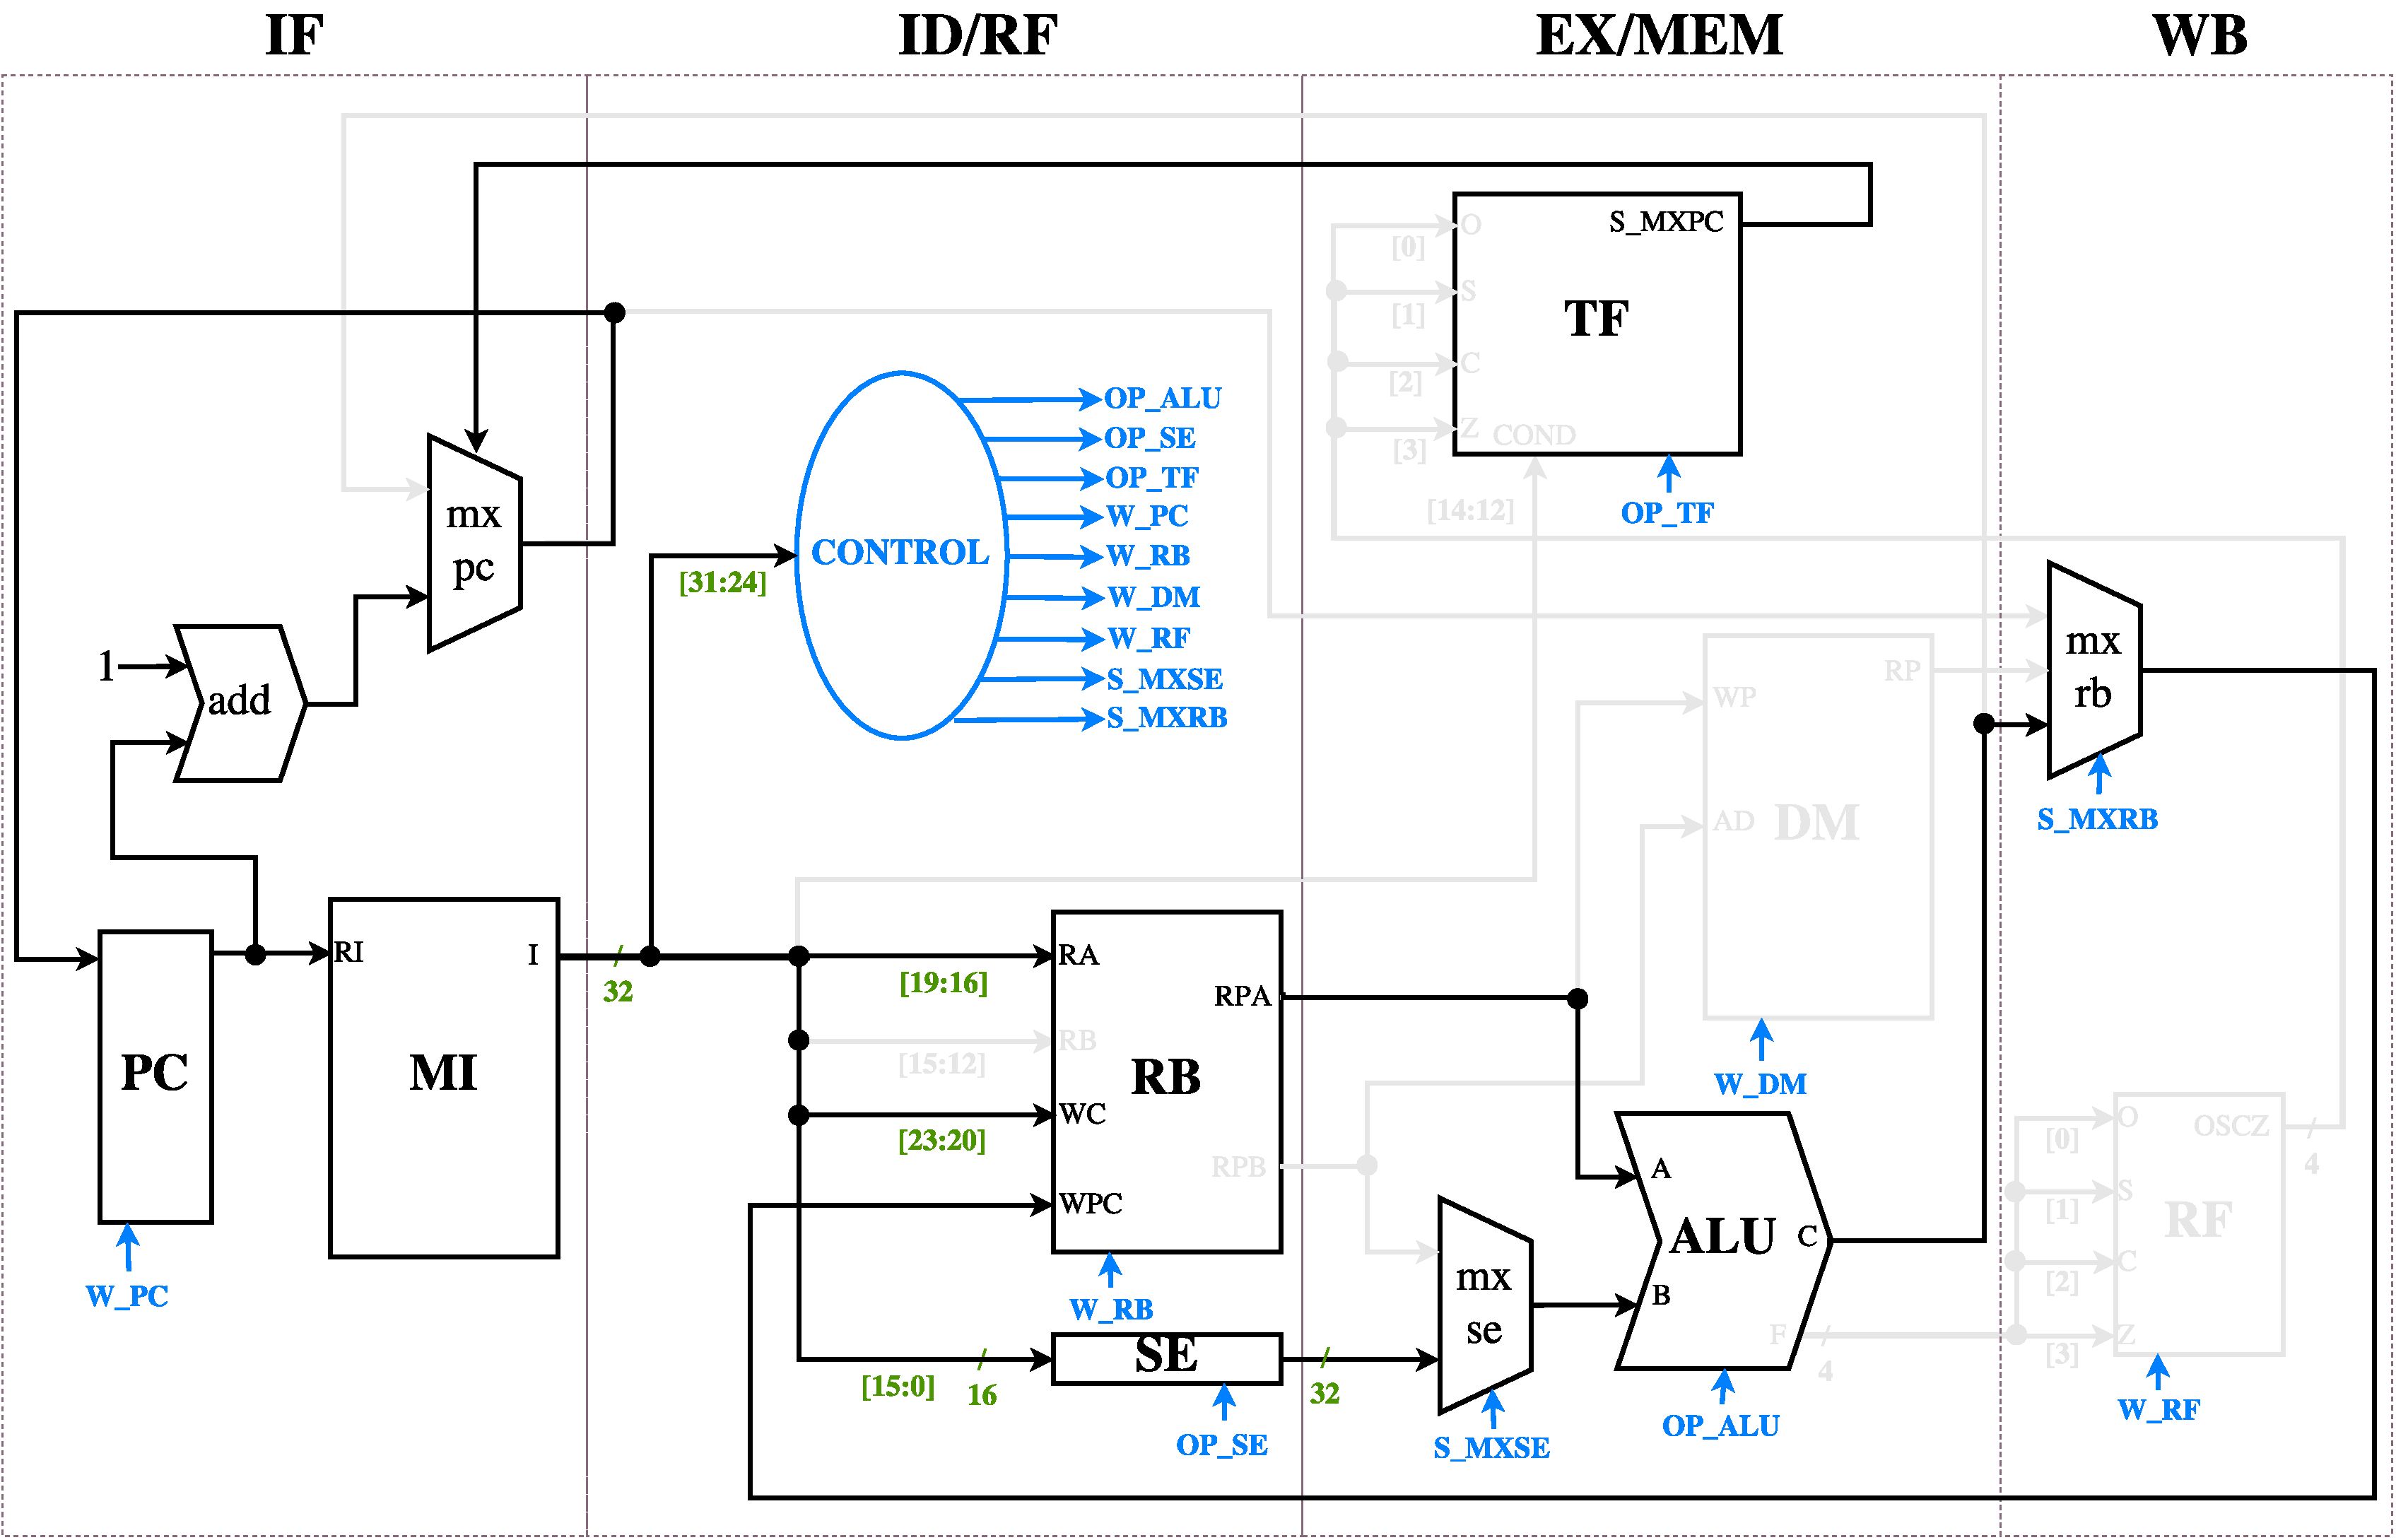
\includegraphics[width=\textwidth]{./pictures/DatapathCONS.pdf}
\caption{Datapath de Constantes}
\end{figure}
A Figura 3 apresenta o caminho de dados específico de instruções com constantes, nela é possível observar quais elementos participam da realização destas operações.\newline

O elemento que caracteriza esse tipo de instrução é o extensor de sinal responsável por transformar uma constante de 16 ou 12 bits em 32 bits. O nível lógico do sinal OP\_SE que define se a constante a ser extendida é de tamanho 12 ou 16. Assim é garantido que o restante dos bits não tenha informações erradas que irão ser operadas na unidade lógica e aritimetica (ALU).

% inicio da tabela de formato de instruções com constante
\FloatBarrier
\begin{table}[H]
  \begin{center}
  \renewcommand{\arraystretch}{1.2}
    \begin{tabular}[pos]{|>{\centering\arraybackslash}m{35pt}|>{\centering\arraybackslash}m{57pt}|>{\centering\arraybackslash}m{46pt}|>{\centering\arraybackslash}m{46pt}|>{\centering\arraybackslash}m{181pt}|} \hline
      \cellcolor[gray]{0.9}\textbf{31:29} & \cellcolor[gray]{0.9}\textbf{28:24} & \cellcolor[gray]{0.9}\textbf{23:20} & \cellcolor[gray]{0.9}\textbf{19:16} & \cellcolor[gray]{0.9}\textbf{15:0} \\ \hline
        0 1 0       & OP        & WC        & X X X X      & CONSTANTE \\ \hline
    \end{tabular}
    \caption{Tabela de Formato}
  \end{center}
\end{table}  
% fim

% inicio da tabela de operações das instruções com constante
\FloatBarrier
\begin{table}[H]
  \begin{center}
  \renewcommand{\arraystretch}{1.2}
    \begin{tabular}[pos]{|>{\centering\arraybackslash}m{80pt}|>{\centering\arraybackslash}m{120pt}|>{\centering\arraybackslash}m{189pt}|} 
      \hline
      \cellcolor[gray]{0.9}\textbf{OPALU} & \cellcolor[gray]{0.9}\textbf{Mnemônico} & \cellcolor[gray]{0.9}\textbf{Operação} \\ \hline
        01100      & loadlit c, Const16        & C = CONSTANTE \\ \hline
        01101      & lcl c, Const16            & C = Const16|(C\&0xffff0000) \\ \hline
        01110      & lch c, Const16            & C = (Const16 « 16)|(C\&0x0000ffff ) \\ \hline
    \end{tabular}
    \caption{Tabela de Instruções com Constante}
  \end{center}
\end{table}  
% fim

\subsection{Instruções de Acesso à Memória}
\begin{figure}[H]
\centering
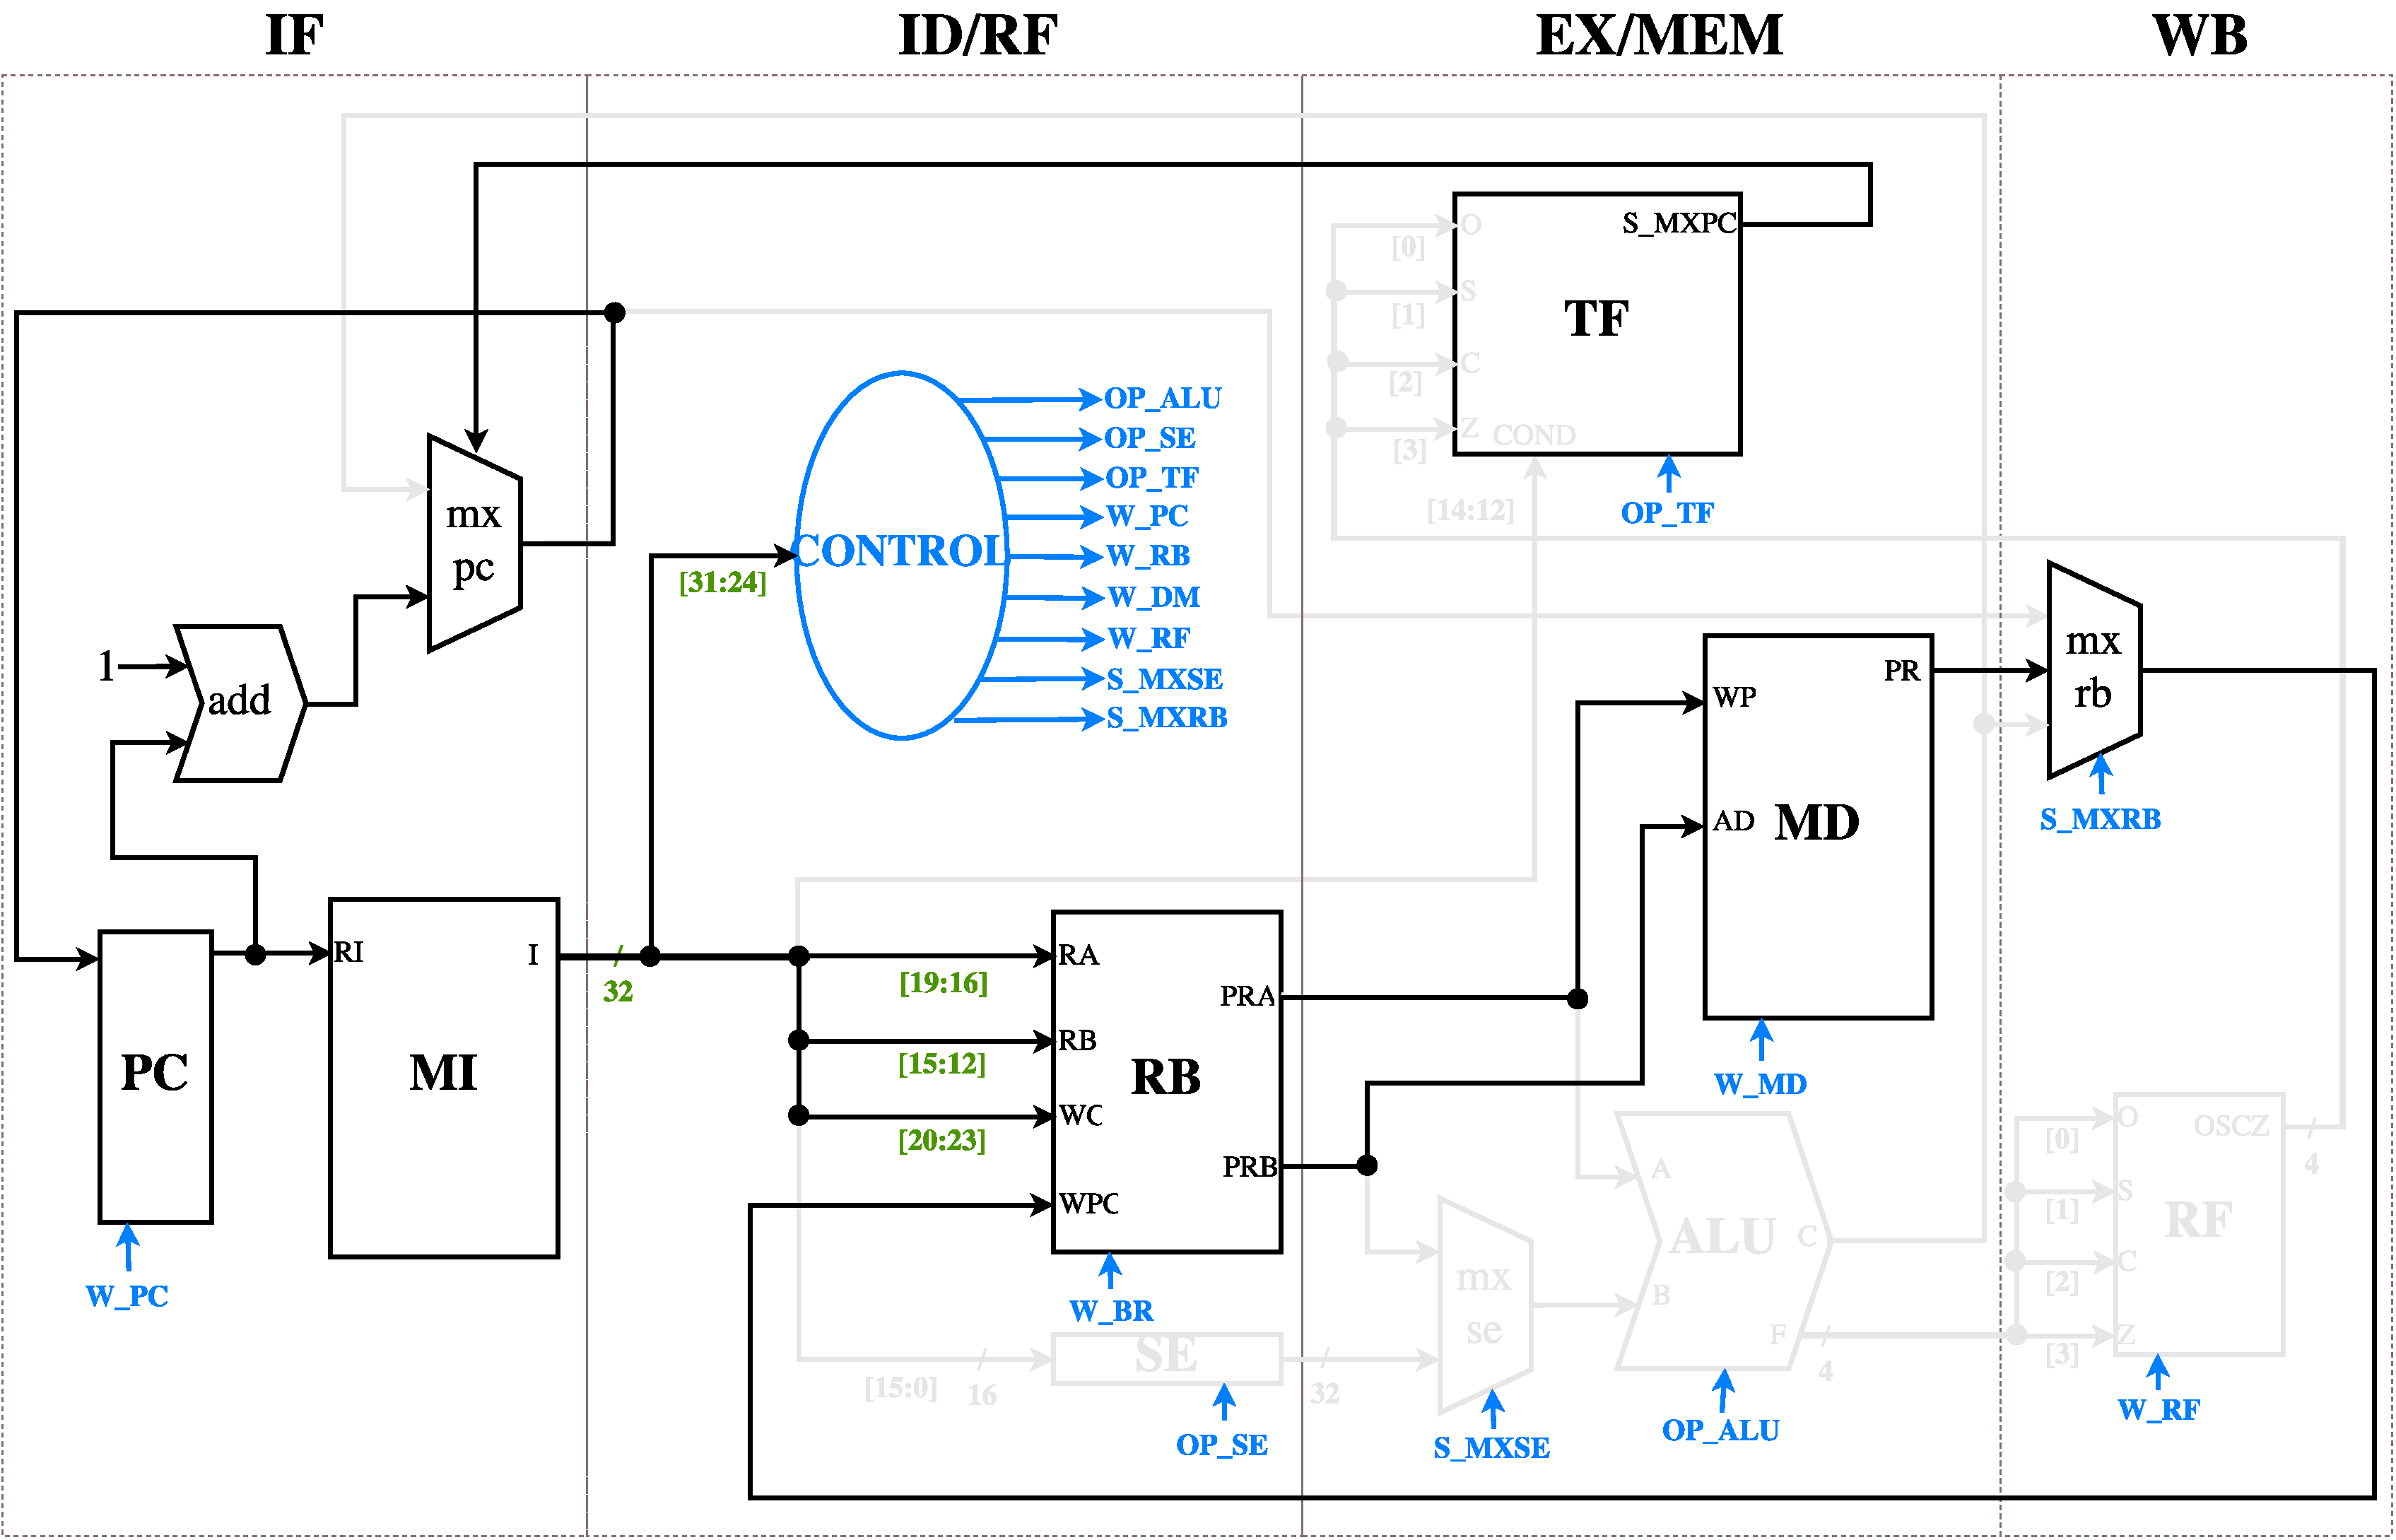
\includegraphics[width=\textwidth]{./pictures/DatapathMEM.pdf}
\caption{Datapath Memória}
\end{figure}

As instruções de acesso à memória são Load e Store. Na instrução Load o endereço presente no registrador B é lido da memória, e a saída é escrita no banco de registradores no endereço especificado na pelo registrador A. Na instrução Store os dados são lidos do banco de registradores e escritos na memória, sendo registrador A o dado a ser escrito e o registrador B endereço onde será armazenado. \newline
O sinal que habilita a escrita na memória de dados é o mesmo que habilita a leitura, quando em nível lógico 1 apenas a escrita é permitida, e em 0, apenas a leitura.
As instruções de acesso à memória possuem o seguinte formato:

% inicio da tabela de formato de instruções de acesso à memória
\FloatBarrier
\begin{table}[H]
  \begin{center}
  \renewcommand{\arraystretch}{1.2}
    \begin{tabular}[pos]{|>{\centering\arraybackslash}m{32pt}|>{\centering\arraybackslash}m{42pt}|>{\centering\arraybackslash}m{22pt}|>{\centering\arraybackslash}m{42pt}|>{\centering\arraybackslash}m{42pt}|>{\centering\arraybackslash}m{42pt}|>{\centering\arraybackslash}m{127pt}|} \hline
      \cellcolor[gray]{0.9}\textbf{31:29} & 
      \cellcolor[gray]{0.9}\textbf{28:25} & 
      \cellcolor[gray]{0.9}\textbf{24} & 
      \cellcolor[gray]{0.9}\textbf{23:20} & 
      \cellcolor[gray]{0.9}\textbf{19:16} & 
      \cellcolor[gray]{0.9}\textbf{15:12} & 
      \cellcolor[gray]{0.9}\textbf{11:0} \\ \hline
      1 0 0         & X X X X &OP & WC        & RA        & RB        & X X X X X X X X X X X X \\ \hline
    \end{tabular}
    \caption{Tabela de Formato}
    \end{center}
\end{table}  
% fim

% inicio da tabela de operações das instruções de acesso à memória
\FloatBarrier
\begin{table}[H]
  \begin{center}
  \renewcommand{\arraystretch}{1.2}
    \begin{tabular}[pos]{|>{\centering\arraybackslash}m{89pt}|>{\centering\arraybackslash}m{160pt}|>{\centering\arraybackslash}m{150pt}|} \hline
      \cellcolor[gray]{0.9}\textbf{OPM} & \cellcolor[gray]{0.9}\textbf{Mnemônico} & \cellcolor[gray]{0.9}\textbf{Operação} \\ \hline
        0       & load c, a         & C = Mem[A] \\ \hline
        1       & store a, b        & Mem[A] = B \\ \hline
    \end{tabular}
    \caption{Tabela de Instruções de Acesso à Memória}
  \end{center}
\end{table}  
% fim


\subsection{Instruções de Desvio}
\begin{figure}[H]
\centering
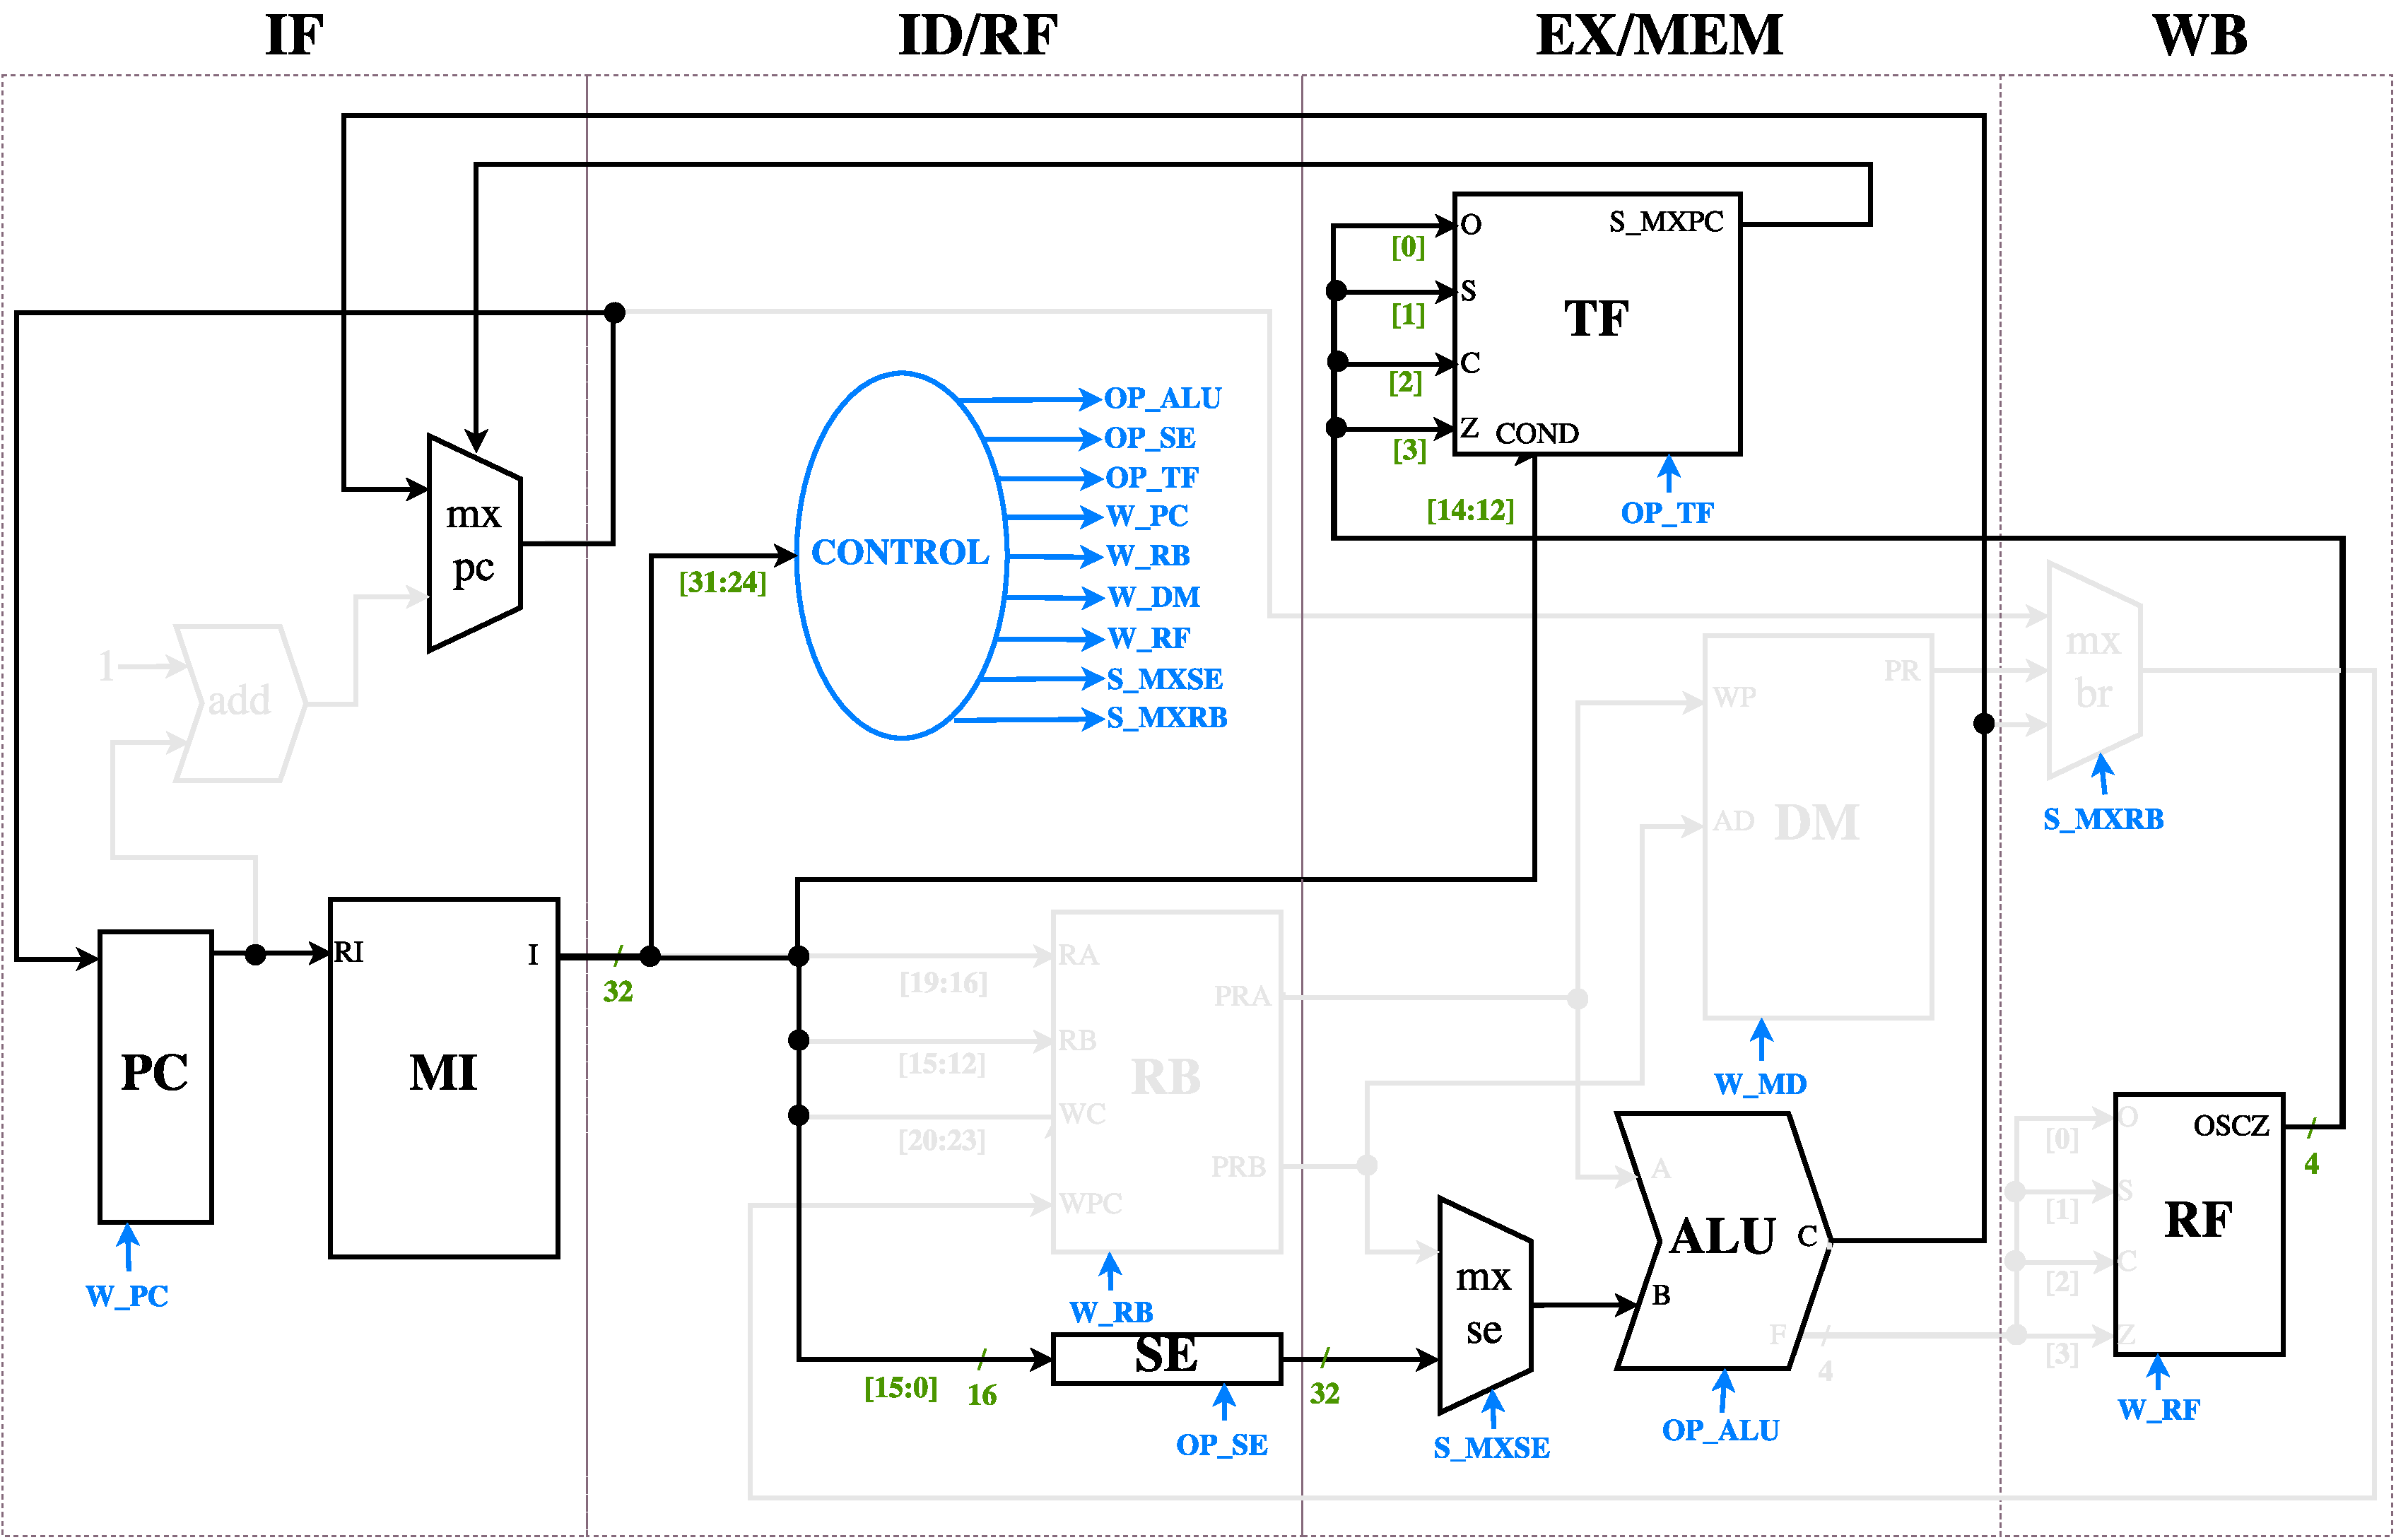
\includegraphics[width=\textwidth]{./pictures/DatapathDES.pdf}
\caption{Datapath Desvio Condicional}
\end{figure}

O módulo que caracteriza essa instrução é o testador de flags (TF) que, a partir de uma condição, determina se um salto será ou não realizado.
As instruções de desvio condicional e incondicional realizam um salto para um endereço absoluto da memória de instruções, informado pelo campo DESTINO. Este endereçamento pode ser de até 2\^{}12 bits. Em caso de endereços maior que 12 bits, deve-se utilizar as instruções lcl e lch para carregar o endereço do Label de destino em um registrador. Em seguida, deve-se realizar um desvio por registrador (especificado na sessão 4.5), utilizando como parâmetro este registrador.
Esta decisão de utilziar endereçamento absoluto retira da ALU a responsabilidade de calcular o novo destino.
\newline
Tais instruções possuem o formato descrito abaixo na tabela:
% inicio da tabela de formato de instruções de desvio
\FloatBarrier
\begin{table}[H]
  \begin{center}
    \begin{tabular}[pos]{|>{\centering\arraybackslash}m{33pt}|>{\centering\arraybackslash}m{28pt}|>{\centering\arraybackslash}m{33pt}|>{\centering\arraybackslash}m{105pt}|>{\centering\arraybackslash}m{33pt}|>{\centering\arraybackslash}m{120pt}|} \hline
      \cellcolor[gray]{0.9}\textbf{31:29} & \cellcolor[gray]{0.9}\textbf{28:27} & \cellcolor[gray]{0.9}\textbf{26:24} & \cellcolor[gray]{0.9}\textbf{23:15} & \cellcolor[gray]{0.9}\textbf{14:12} & \cellcolor[gray]{0.9}\textbf{11:0} \\ \hline
        000       & X X       & OPTF       & X X X X X X X X X      & COND       & DESTINO \\ \hline
    \end{tabular}
    \caption{Tabela de Formato}
  \end{center}
\end{table}  
% fim

% inicio da tabela de operações das instruções de desvio
\FloatBarrier
\begin{table}[H]
  \begin{center}
    \begin{tabular}[pos]{|>{\centering\arraybackslash}m{50pt}|>{\centering\arraybackslash}m{130pt}|>{\centering\arraybackslash}m{209pt}|} \hline
      \cellcolor[gray]{0.9}\textbf{OPD} & \cellcolor[gray]{0.9}\textbf{Mnemônico} & \cellcolor[gray]{0.9}\textbf{Operação} \\ \hline
        000      & jf.cond DESTINO            & Jump False \\ \hline
        001      & jt.cond DESTINO       & Jump True \\ \hline
        010      & j DESTINO       & Jump Incondicional \\ \hline
    \end{tabular}
    \caption{Tabela de Instruções de Desvio}
  \end{center}
\end{table}  
% fim

As instruções de desvio condicional devem testar as condições apresentadas no quadro abaixo:

% inicio da tabela de condições
\FloatBarrier
\begin{table}[H]
  \begin{center}
    \begin{tabular}[pos]{|>{\centering\arraybackslash}m{70pt}|>{\centering\arraybackslash}m{130pt}|>{\centering\arraybackslash}m{189pt}|} \hline
      \cellcolor[gray]{0.9}\textbf{COND} & \cellcolor[gray]{0.9}\textbf{Mnemônico} & \cellcolor[gray]{0.9}\textbf{Condição}  \\ \hline
        000         & true          & TRUE \\ \hline
        001         & neg           & Resultado da ALU negativo \\ \hline
        010         & zero          & Resultado da ALU zero \\ \hline
        100         & carry         & Carry da ALU \\ \hline
        101         & negzero       & Resultado da ALU negativo ou zero \\ \hline
        111         & overflow      & Resultado da ALU overflow \\ \hline
    \end{tabular}
    \caption{Tabela de Condições}
  \end{center}
\end{table}  

% fim
\newpage
\subsection{Instruções de Desvio por Registrador}
\begin{figure}[H]
\centering
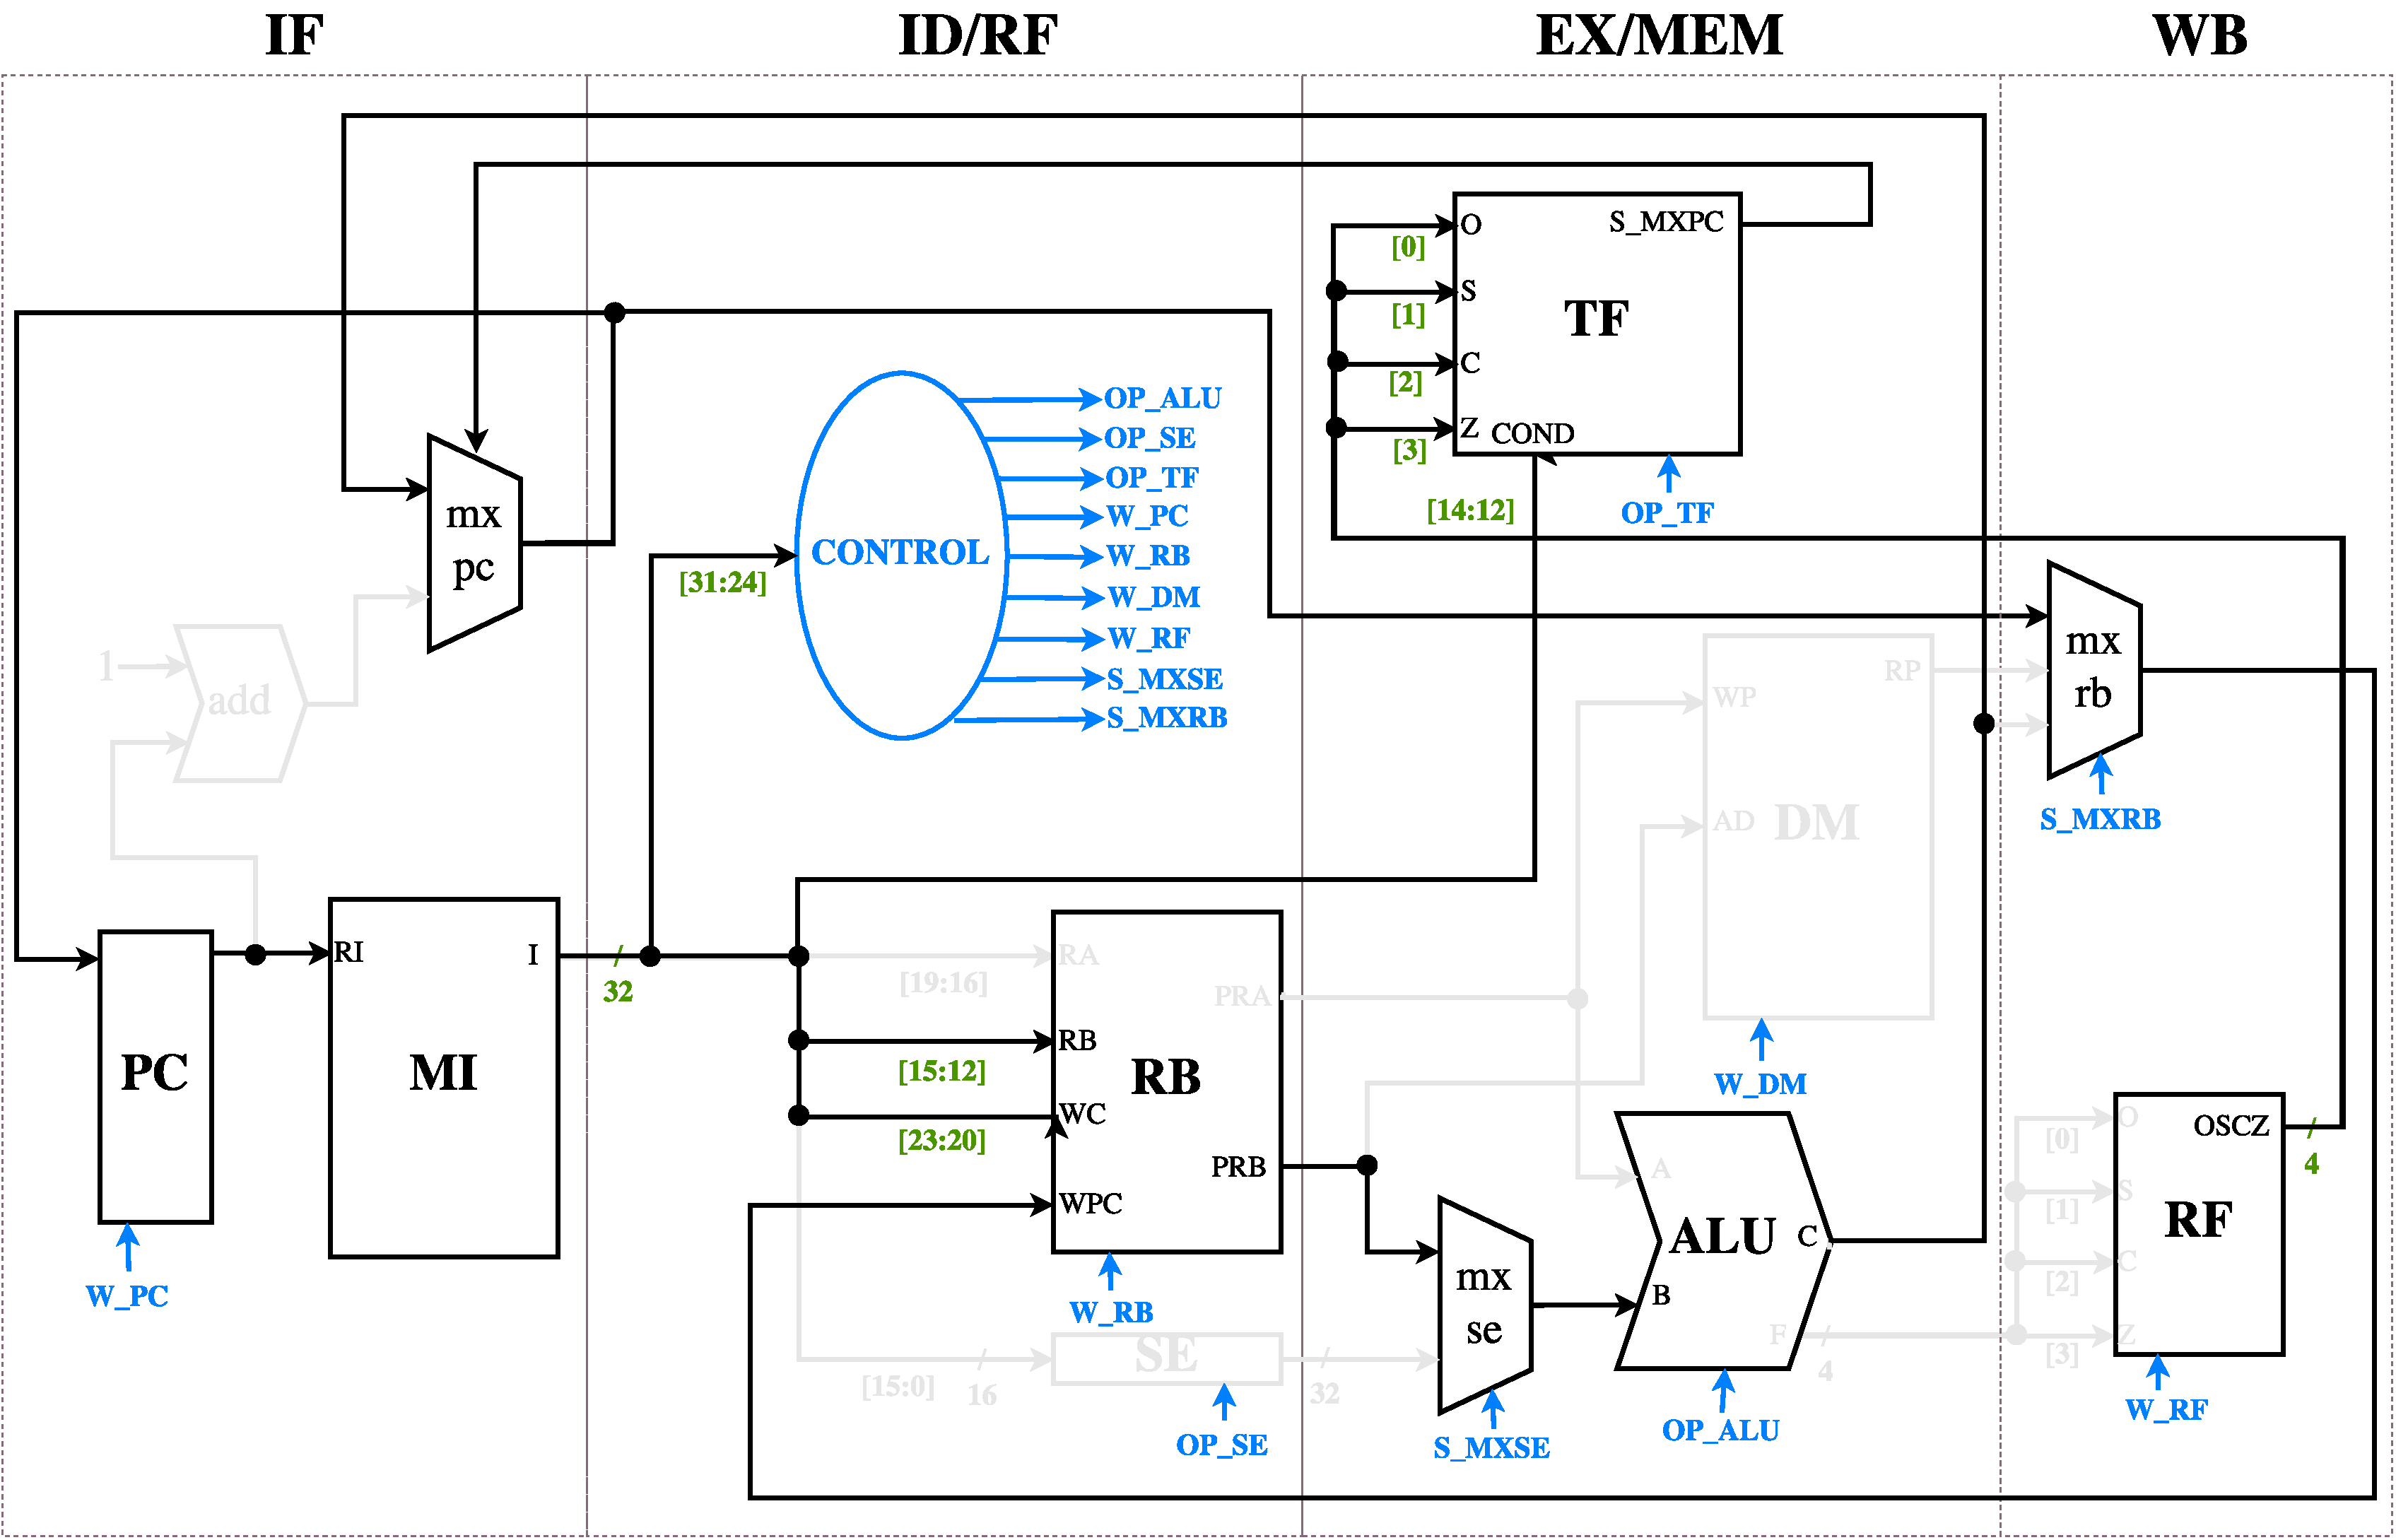
\includegraphics[width=\textwidth]{./pictures/DatapathDER.pdf}
\caption{Datapath Desvio por Registrador}
\end{figure}
São duas as instruções de desvio por registrador, jump and link e jump register. Na instrução de jump and link, o valor de PC+1 deve ser armazenado no registrador r15 (definido pela unidade de controle) e o conteúdo do registrador RB armazenado em PC. Já no caso da instrução jump register, a única operação a ser feita é armazenar o conteúdo do registrador RB no PC.\newline

As instruções de desvio por registrador possuem o seguinte formato:

% inicio da tabela de formato de instruções de desvio por registrador
\FloatBarrier
\begin{table}[H]
  \begin{center}
  \renewcommand{\arraystretch}{1.46}
    \begin{tabular}[pos]{|>{\centering\arraybackslash}m{31pt}|>{\centering\arraybackslash}m{32pt}|>{\centering\arraybackslash}m{29pt}|>{\centering\arraybackslash}m{90pt}|>{\centering\arraybackslash}m{32pt}|>{\centering\arraybackslash}m{127pt}|} \hline
      \cellcolor[gray]{0.9}\textbf{31:29} & \cellcolor[gray]{0.9}\textbf{28:27} & \cellcolor[gray]{0.9}\textbf{26:24} & \cellcolor[gray]{0.9}\textbf{23:16} & \cellcolor[gray]{0.9}\textbf{15:12} & \cellcolor[gray]{0.9}\textbf{11:0} \\ \hline
        1 1 0       & X X       & OPDR       & X X X X X X X X       & RB        & X X X X X X X X X X X X \\ \hline
    \end{tabular}
    \caption{Tabela de Formato}
  \end{center}
\end{table}  
% fim

% inicio da tabela 
\FloatBarrier
\begin{table}[H]
  \begin{center}
  \renewcommand{\arraystretch}{1.46}
    \begin{tabular}[pos]{|>{\centering\arraybackslash}m{89pt}|>{\centering\arraybackslash}m{150pt}|>{\centering\arraybackslash}m{150pt}|} \hline
      \cellcolor[gray]{0.9}\textbf{OPDR} & \cellcolor[gray]{0.9}\textbf{Mnemônico} & \cellcolor[gray]{0.9}\textbf{Operação} \\ \hline
        011       & jal b         & Jump and Link \\ \hline
        100       & jr b          & Jump Register \\ \hline
    \end{tabular}
    \caption{Tabela de Instruções de Desvio por Registrador}
  \end{center}
\end{table}  
% fim

\subsection{HALT}
A instrução HALT representa uma parada no sistema.\newline

O HALT possui o formato seguinte:

% inicio da tabela de formato do HALT
\FloatBarrier
\begin{table}[H]
  \begin{center}
    \begin{tabular}[pos]{|>{\centering\arraybackslash}m{34pt}|>{\centering\arraybackslash}m{30pt}|>{\centering\arraybackslash}m{34pt}|>{\centering\arraybackslash}m{136pt}|>{\centering\arraybackslash}m{130pt}|} \hline
      \cellcolor[gray]{0.9}\textbf{31:29} & \cellcolor[gray]{0.9}\textbf{28:27} & \cellcolor[gray]{0.9}\textbf{26:24} & \cellcolor[gray]{0.9}\textbf{23:12} & \cellcolor[gray]{0.9}\textbf{11:0}  \\ \hline
        1 0 1       & X X       & 00        & X X X X X X X X X X X X       & L \\ \hline
    \end{tabular}
    \caption{Tabela de Formato}
  \end{center}
\end{table}  
% fim

% inicio da tabela de operação HALT
\FloatBarrier
\begin{table}[H]
  \begin{center}
    \begin{tabular}[pos]{|>{\centering\arraybackslash}m{182pt}|>{\centering\arraybackslash}m{220pt}|} \hline
      \cellcolor[gray]{0.9}\textbf{Mnemônico} & \cellcolor[gray]{0.9}\textbf{Operação} \\ \hline
        L: j L      & PC = PC \\ \hline
    \end{tabular}
    \caption{Tabela de Instrução HALT}
  \end{center}
\end{table}  
% fim

\subsection{NOP}
Nessa instrução todos os sinais de controle são zerados, desta forma nada é registrado na memória ou no banco de registradores. A NOP possui o formato seguinte:

% inicio da tabela de formato do NOP
\FloatBarrier
\begin{table}[H]
  \begin{center}
    \begin{tabular}[pos]{|>{\centering\arraybackslash}m{37pt}|>{\centering\arraybackslash}m{365pt}|} \hline
    \cellcolor[gray]{0.9}\textbf{31:29} & \cellcolor[gray]{0.9}\textbf{28:0} \\ \hline
        0 0 0       &  X X X X X X X X X X X X X X X X X X X X X X X X X X X X X \\ \hline
    \end{tabular}
    \caption{Tabela de Formato}
  \end{center}
\end{table}  
% fim

\newpage
\section{Descrição dos Componentes}
Durante algumas discussões foi decidido quais  componentes constituiriam o processador. A partir de análises das instruções foram listados os componentes a seguir:
\subsection{Contador de Programa (Program Counter)}
O Contador de Programa (PC) é o registrador que armazena o endereço da próxima instrução a ser executada. Ele é atualizado assim que a instrução atual é finalizada.
\begin{figure}[H]
\centering
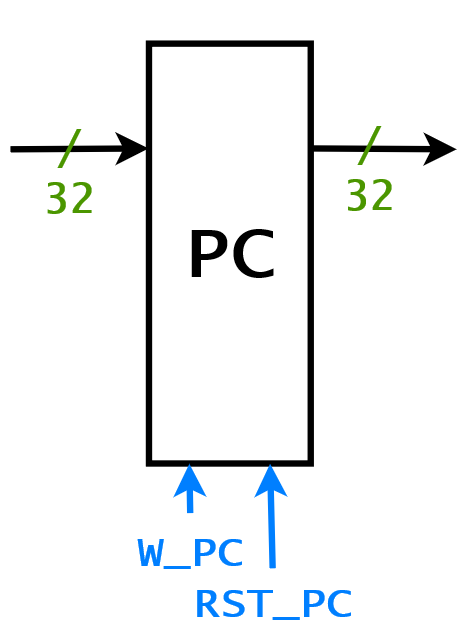
\includegraphics[width=0.25\textwidth]{./pictures/PC.PNG}
\caption{Contador de Programa}
\end{figure}

% inicio da tabela
\FloatBarrier
\begin{table}[H]
  \begin{center}
  \renewcommand{\arraystretch}{1.15}
    \begin{tabular}[pos]{|>{\centering\arraybackslash}m{50pt}|>{\centering\arraybackslash}m{60pt}|>{\centering\arraybackslash}m{70pt}|>{\centering\arraybackslash}m{182pt}|} \hline
      \cellcolor[gray]{0.9}\textbf{Nome} & 
      \cellcolor[gray]{0.9}\textbf{Tamanho} & 
      \cellcolor[gray]{0.9}\textbf{Direção} &
      \cellcolor[gray]{0.9}\textbf{Descrição} \\ \hline
        in\_PC      & 32    & Entrada   & Endereço de destino do salto \\ \hline
        out\_PC     & 32    & Saída     & Saída do PC \\ \hline
        W\_PC       & 1     & Entrada   & Sinal de controle do PC\\ \hline
        RST\_PC     & 1     & Entrada   & Sinal que limpa o pc\\ \hline
    \end{tabular}
    \caption{Tabela de Sinais do PC}
  \end{center}
\end{table}  
% fim

\subsection{Memória de Instruções}
Tem como funcionalidade armazenar todas as instruções do programa a ser executado. 

\begin{figure}[H]
\centering
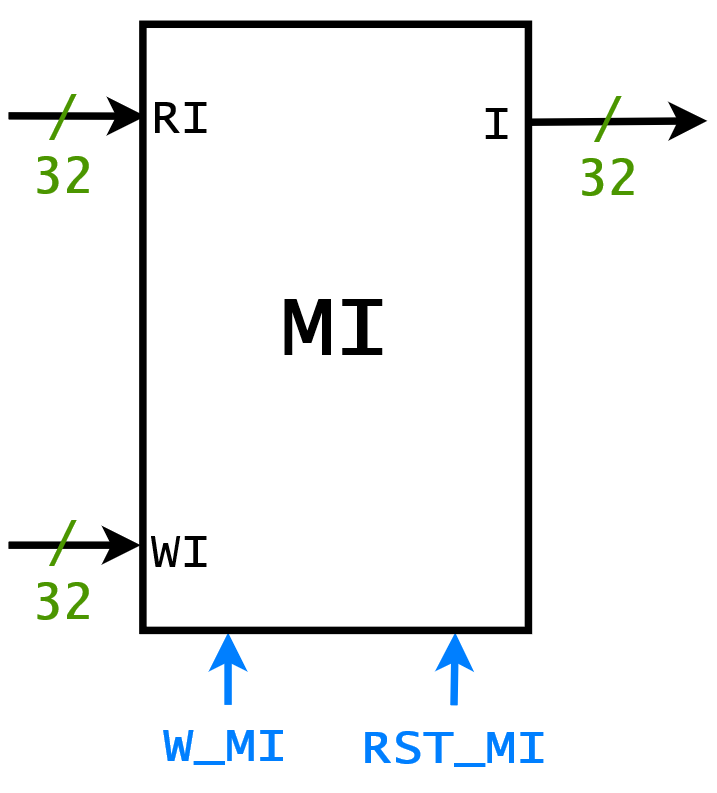
\includegraphics[width=0.3\textwidth]{./pictures/MI.PNG}
\caption{Memória de Instruções}
\end{figure}

% inicio da tabela
\FloatBarrier
\begin{table}[H]
  \begin{center}
  \renewcommand{\arraystretch}{1.1}
    \begin{tabular}[pos]{|>{\centering\arraybackslash}m{50pt}|>{\centering\arraybackslash}m{60pt}|>{\centering\arraybackslash}m{70pt}|>{\centering\arraybackslash}m{182pt}|} \hline
      \cellcolor[gray]{0.9}\textbf{Nome} & 
      \cellcolor[gray]{0.9}\textbf{Tamanho} & 
      \cellcolor[gray]{0.9}\textbf{Direção} &
      \cellcolor[gray]{0.9}\textbf{Descrição} \\ \hline
       RI       & 32 & Entrada & Endereço da instrução a ser lida\\ \hline
       WI       & 32 & Entrada & Endereço de entrada na memória de instrução \\ \hline
       I        & 32 & Saída   & Instrução atual \\ \hline
       W\_MI    & 1 & Entrada  & Sinal que habilita a leitura \\ \hline
       RST\_MI  & 1 & Entrada  & Sinal que limpa a memória de instruções \\ \hline
       
    \end{tabular}
    \caption{Tabela de Sinais da Memória de Instruções}
  \end{center}
\end{table}  
% fim

\subsection{Banco de Registradores}
O banco de registradores consiste em um bloco formado por 16 registradores de propósito geral de 32 bits.

\begin{figure}[H]
\centering
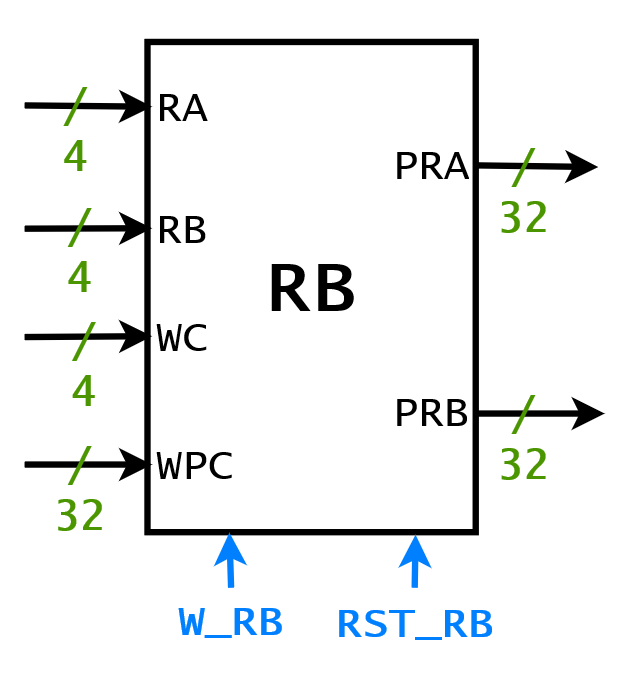
\includegraphics[width=0.3\textwidth]{./pictures/RB.PNG}
\caption{Banco de Registradores}
\end{figure}

% inicio da tabela
\FloatBarrier
\begin{table}[H]
  \begin{center}
  \renewcommand{\arraystretch}{1.1}
    \begin{tabular}[pos]{|>{\centering\arraybackslash}m{50pt}|>{\centering\arraybackslash}m{60pt}|>{\centering\arraybackslash}m{70pt}|>{\centering\arraybackslash}m{182pt}|} \hline
      \cellcolor[gray]{0.9}\textbf{Nome} & 
      \cellcolor[gray]{0.9}\textbf{Tamanho} & 
      \cellcolor[gray]{0.9}\textbf{Direção} &
      \cellcolor[gray]{0.9}\textbf{Descrição} \\ \hline
       RA     & 4   & Entrada   & Endereço do registrador A \\ \hline
       RB     & 4   & Entrada   & Endereço do registrador B \\ \hline
       WC     & 4   & Entrada   & Endereço de escrita para o registrador destino \\ \hline
       WPC    & 32  & Entrada   & Entrada do dado a ser armazenado no registrador destino \\ \hline
       PRA & 32 & Saída & Saída do registrador A \\ \hline
       PRB & 32 & Saída & Saída do registrador B \\ \hline
       W\_RB & 1 & Entrada & Sinal que habilita a escrita no banco de resgistradores \\ \hline
       RST\_RB  & 1 & Entrada  & Sinal que limpa a memória de instruções \\ \hline
    \end{tabular}
    \caption{Tabela de Sinais do Banco de Registradores}
  \end{center}
\end{table}  
% fim

\subsection{Extensor de Sinal}
O extensor de sinal é utilizado para extender o sinal dos bits de entrada nas operações com constantes e operações de desvio.
\newline\newline
\begin{figure}[H]
\centering
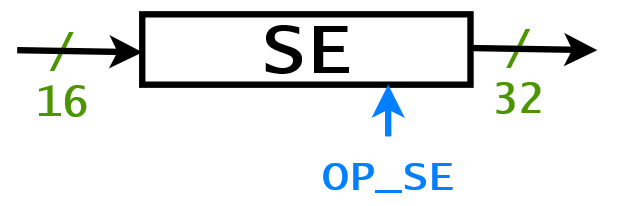
\includegraphics[width=0.3\textwidth]{./pictures/SE.PNG}
\caption{Extensor de Sinais}
\end{figure}
% inicio da tabela
\FloatBarrier
\begin{table}[H]
  \begin{center}
  \renewcommand{\arraystretch}{1.5}
    \begin{tabular}[pos]{|>{\centering\arraybackslash}m{50pt}|>{\centering\arraybackslash}m{60pt}|>{\centering\arraybackslash}m{70pt}|>{\centering\arraybackslash}m{182pt}|} \hline
      \cellcolor[gray]{0.9}\textbf{Nome} & 
      \cellcolor[gray]{0.9}\textbf{Tamanho} & 
      \cellcolor[gray]{0.9}\textbf{Direção} &
      \cellcolor[gray]{0.9}\textbf{Descrição} \\ \hline
       InSE & 16 &  Entrada  & Constante a ser extendida \\ \hline
       InSE & 12 &  Entrada  & Constante a ser extendida \\ \hline
       OutSE & 32 &  Saída  & Constante extendida \\ \hline
       OP\_SE & 1  &  Entrada  & Sinal de controle do extensor \\ \hline
    \end{tabular}
    \caption{Tabela de Sinais do Extensor de Sinais}
  \end{center}
\end{table}  
% fim
\subsection{Unidade Lógica e Aritmética (Arithmetic Logic Unit)}
A ALU é um circuito combinacional responsável por realizar operações aritméticas e lógicas dentro do processador. As operações a serem executadas são determinadas por meio dos sinais de controle e das suas entradas de operação, logo após os dados de entrada são computados e o resultado é obtido na saída do circuito.
\newline\newline

\begin{figure}[H]
\centering
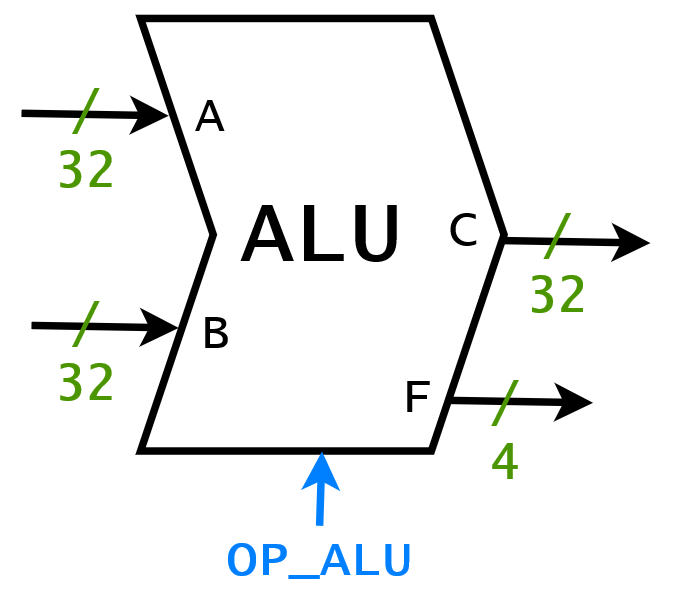
\includegraphics[width=0.3\textwidth]{./pictures/ALU.PNG}
\caption{Unidade Lógica Aritmética}
\end{figure}
\newpage

% inicio da tabela
\FloatBarrier
\begin{table}[H]
  \begin{center}
  \renewcommand{\arraystretch}{1.1}
    \begin{tabular}[pos]{|>{\centering\arraybackslash}m{50pt}|>{\centering\arraybackslash}m{60pt}|>{\centering\arraybackslash}m{70pt}|>{\centering\arraybackslash}m{182pt}|} \hline
      \cellcolor[gray]{0.9}\textbf{Nome} & 
      \cellcolor[gray]{0.9}\textbf{Tamanho} & 
      \cellcolor[gray]{0.9}\textbf{Direção} &
      \cellcolor[gray]{0.9}\textbf{Descrição} \\ \hline
        A       &   32 & Entrada   & Operando A \\ \hline
        B       &   32 & Entrada   & Operando B \\ \hline
        C       &   32 & Saída     & Resultado da operação \\ \hline
        F       &   4  & Saída     & Flags  \\ \hline
        OP\_ALU  &   5  & Entrada   & Código de operação da instrução atual  \\ \hline
    \end{tabular}
    \caption{Tabela de sinais da ALU}
  \end{center}
\end{table}  
% fim

\subsection{Memória de Dados (Data Memory)}
A Memória de dados tem como propósito salvar/ler dados proveniente das instruções de acesso à memória. 

\begin{figure}[H]
\centering
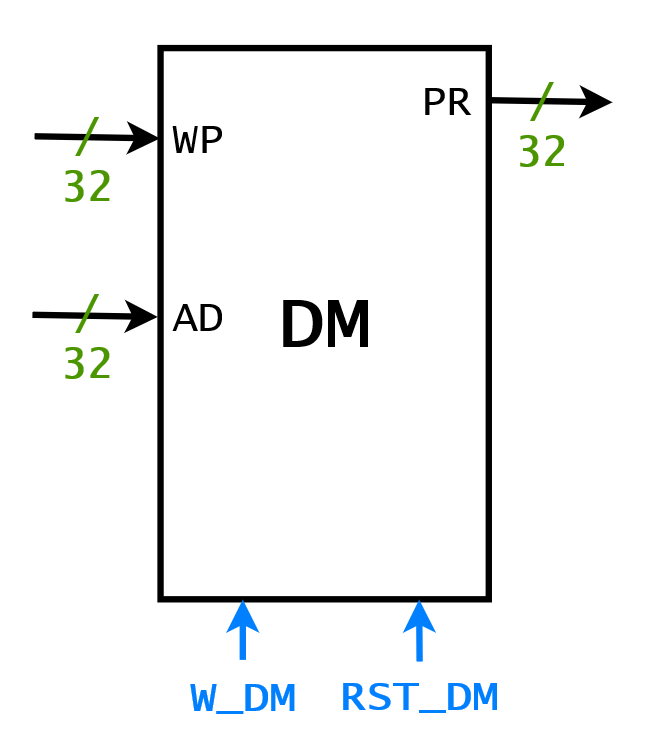
\includegraphics[width=0.3\textwidth]{./pictures/DM.PNG}
\caption{Memória de Dados}
\end{figure}

% inicio da tabela
\FloatBarrier
\begin{table}[H]
  \begin{center}
  \renewcommand{\arraystretch}{1.3}
    \begin{tabular}[pos]{|>{\centering\arraybackslash}m{50pt}|>{\centering\arraybackslash}m{60pt}|>{\centering\arraybackslash}m{70pt}|>{\centering\arraybackslash}m{182pt}|} \hline
      \cellcolor[gray]{0.9}\textbf{Nome} & 
      \cellcolor[gray]{0.9}\textbf{Tamanho} & 
      \cellcolor[gray]{0.9}\textbf{Direção} &
      \cellcolor[gray]{0.9}\textbf{Descrição} \\ \hline
       WP  & 32  & Entrada   & Dado as ser armazenado na memória \\ \hline
       AD  & 32  & Entrada   & Endereço onde o dado será armazenado \\ \hline
       PR  & 32  & Saída     & Dado que sai da memória e é escrito no registrador \\ \hline
       W\_DM & 1 & Entrada   & Sinal que habilita a escrita na memória de dados \\ \hline
       RST\_DM & 1 & Entrada   & Sinal que limpa a memória de dados \\ \hline
    \end{tabular}
    \caption{Tabela de Sinais da Memória de Dados}
  \end{center}
\end{table}  
% fim

\subsection{Registrador de Flags}
Responsável por armazenar os estados das flags Overflow, Carry, Sinal e Zero. Estes estados são atualizados de acordo com o tipos e resultados das operações realizadas pela unidade lógica e aritmética. 

\begin{figure}[H]
\centering
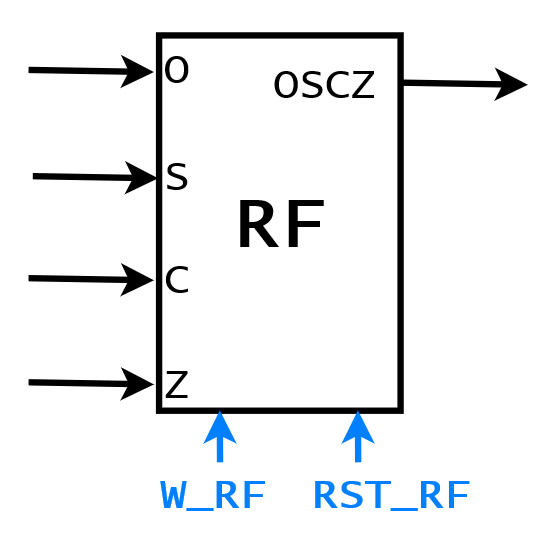
\includegraphics[width=0.3\textwidth]{./pictures/RF.PNG}
\caption{Registrador de Flags}
\end{figure}

% inicio da tabela
\FloatBarrier
\begin{table}[H]
  \begin{center}
  \renewcommand{\arraystretch}{1.4}
    \begin{tabular}[pos]{|>{\centering\arraybackslash}m{50pt}|>{\centering\arraybackslash}m{60pt}|>{\centering\arraybackslash}m{70pt}|>{\centering\arraybackslash}m{182pt}|} \hline
      \cellcolor[gray]{0.9}\textbf{Nome} & 
      \cellcolor[gray]{0.9}\textbf{Tamanho} & 
      \cellcolor[gray]{0.9}\textbf{Direção} &
      \cellcolor[gray]{0.9}\textbf{Descrição} \\ \hline
        O    &   1   & Entrada & Flag de overflow \\ \hline
        S    &   1   & Entrada & Flag de sinal\\ \hline
        C    &   1   & Entrada & Flag de carry\\ \hline
        Z    &   1   & Entrada & Flag de zero \\ \hline
        OSCZ &   4   & Saída   & Flags atualizadas \\ \hline
        W\_RF &  3   & Entrada & Sinal que define quais flags serão atualizada \\ \hline
        RST\_RF & 1   & Entrada & Limpa os dados do registrador \\ \hline
    \end{tabular}
    \caption{Tabela de Sinais do Registrador de Flags}
  \end{center}
\end{table}  
% fim

\subsection{Testador de Flags}
Esse módulo combinacional foi criado com o objetivo de decidir se um jump será ou não realizado conforme a condição (COND).O testador verifica se uma determinada flag esta no estado desejado.

\begin{figure}[H]
\centering
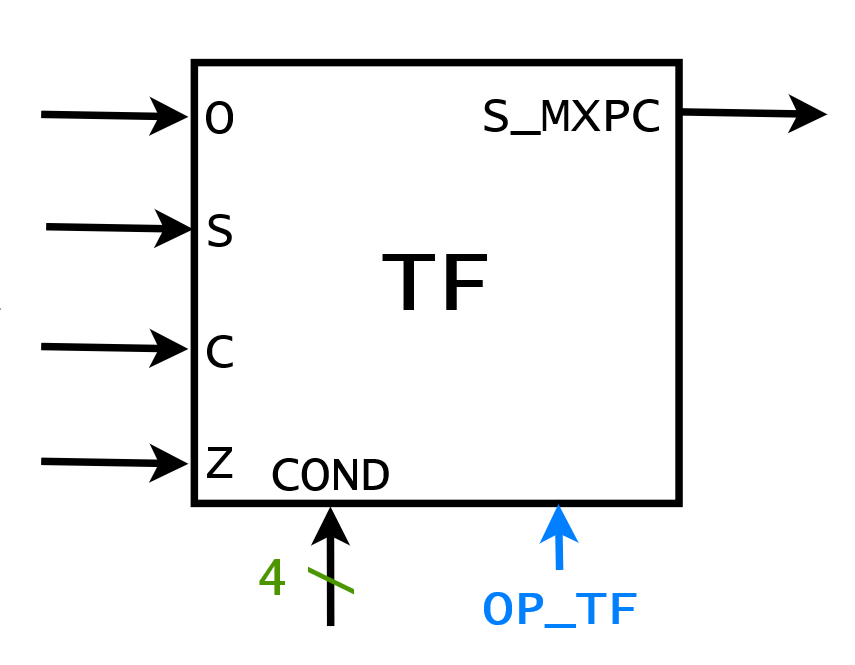
\includegraphics[width=0.3\textwidth]{./pictures/TF.PNG}
\caption{Testador de Flags}
\end{figure}
% inicio da tabela
\FloatBarrier
\begin{table}[H]
  \begin{center}
  \renewcommand{\arraystretch}{1.15}
    \begin{tabular}[pos]{|>{\centering\arraybackslash}m{50pt}|>{\centering\arraybackslash}m{60pt}|>{\centering\arraybackslash}m{70pt}|>{\centering\arraybackslash}m{182pt}|} \hline
      \cellcolor[gray]{0.9}\textbf{Nome} & 
      \cellcolor[gray]{0.9}\textbf{Tamanho} & 
      \cellcolor[gray]{0.9}\textbf{Direção} &
      \cellcolor[gray]{0.9}\textbf{Descrição} \\ \hline
       O    &   1   & Entrada & Flag de overflow a ser testada \\ \hline
        S    &   1   & Entrada & Flag de sinal a ser testada\\ \hline
        C    &   1   & Entrada & Flag de carry a ser testada\\ \hline
        Z    &   1   & Entrada & Flag de zero a ser testada \\ \hline
        COND &   3   & Entrada &Condição que será testada \\ \hline
        S\_MXPC  &   1   & Saída & Sinal que indica se o salto será ou não realizado \\
        \hline
        OP\_TF & 1  &  Entrada  & Sinal de controle do testador de flags \\ \hline
    \end{tabular}
    \caption{Tabela de Sinais do Testador de Flags}
  \end{center}
\end{table}  
% fim

\subsection{Unidade de Controle}
Esta unidade é responsável por gerar todos os sinais que controlam o fluxo das tarefas dentro do processador, sinais estes que permitem a leitura ou escrita em registradores, controle de barramento por meio de multiplexadores e códigos de operação para módulos combinacionais.

A unidade de controle é implementada no modelo hardwired, que tem como sua característica principal uma máquina de estado finita (FSM), que seus estados são definidos pelos estágios do processador (IF,ID,EX/MEM,WB). A cada estado todos os sinais de controle são redefinidos afim de controla todos os elementos para realizar a tarefa desejada.

Esse modelo de implementação tem melhor desempenho em relação ao modelo microprogramada, pois a microprogramada é composta por uma memoria de microprograma, o que lhe da a capacidade de reprograma-la sem precisar reestruturar o circuito. Por outro lado projetar uma unidade de controle hardwired é mais dificil que microprogramada. Porém em geral no modelo RISC, como formato de instrução é mais simples, utiliza-se o modelo hardwired.[

% inicio da tabela
\begin{center}
\begin{longtable}[pos]{|>{\centering\arraybackslash}m{50pt}|>{\centering\arraybackslash}m{60pt}|>{\centering\arraybackslash}m{70pt}|>{\centering\arraybackslash}m{182pt}|} \hline
	\cellcolor[gray]{0.9}\textbf{Nome} & \cellcolor[gray]{0.9}\textbf{Tamanho} & \cellcolor[gray]{0.9}\textbf{Direção} & \cellcolor[gray]{0.9}\textbf{Descrição}\\ \hline \endfirsthead \hline
	\multicolumn{4}{|c|}{{\bfseries \textbf{continuação da tabela anterior}}} \\ \hline
	\cellcolor[gray]{0.9}\textbf{Nome} & \cellcolor[gray]{0.9}\textbf{Tamanho} & \cellcolor[gray]{0.9}\textbf{Direção} & \cellcolor[gray]{0.9}\textbf{Descrição}\\ \hline \endhead
	\multicolumn{4}{|c|}{{\textbf{continua na próxima página}}} \\ \hline \endfoot
	\hline \endlastfoot
	
	
    TYPE\_OP      &  8  & Entrada & Instrução atual \\ \hline
    OP\_ALU       &  5   & Saída   & Código de operação da instrução atual \\ \hline
    OP\_SE        &  1   & Saída   & Sinal de controle do extensor de sinais. Sendo 0 extende de 12 para 32, sendo 1 extende de 16 para 32 \\ \hline
    OP\_TF        &  3   & Saída   & Sinal que indica se o jump é true ou false \\ \hline
    W\_PC         &  1   & Saída   & Sinal de controle do PC \\ \hline
    W\_RB         &  1   & Saída   & Sinal que habilita a escrita no banco de registradores \\ \hline
    W\_DM         &  1   & Saída   & Sinal que habilita a escrita na memória de dados \\ \hline
    W\_RF         &  1   & Saída   & Sinal que habilita o registrador de flags \\ \hline
    S\_MXSE       &  1   & Saída   & Sinal que controla o multiplexador MXSE. Sendo 1, habilita para a saída do mux o valor de saída do SE, sendo 0, habilita para a saída do mux o valor do registrador B do banco de registradores.   \\ \hline
    S\_MXRB       &  2   & Saída   & Sinal que controla o multiplexador MXRB. Sendo 11, habilita para a saída do mux o valor da saída da ULA, sendo 10, habilita para a saída a saída da memória de dados e sendo 01, habilita para a saída do mux o valor de PC.  \\ \hline
    
    \caption{Tabela de Sinais da Unidade de Controle}
\end{longtable}
\end{center}
% fim

%Como esta arquitetura é baseada em RISC e o projeto exige um processador que faça juízo ao nome LAPIDOPACALAMBA, a unidade de controle será implementada em hardwired.

\newpage
\section{Assembly}
Para a codificação dos programas deve ser utilizada a linguagem Assembly. Através dos mnemônicos já descritos anteriormente, serão escritas as instruções a serem executadas. Em seguida, através de um programa montador, o código fonte do programa será traduzido em linguagem de máquina para um arquivo binário que poderá ser entendido pelo processador e executado.\newline

Além das instruções, o código fonte deve/pode conter algumas diretivas importantes, são elas:

\begin{itemize}
\item \textbf .module NOME - Indica o início do programa com o nome informado;
\item \textbf .pseg - Indica o segmento de programa, ou seja, a partir desse ponto devem conter as instruções a serem executadas. Esta diretiva é encerrada após a ocorrência de uma das diretivas seguintes;
\item \textbf .dseg - Indica o segmento de dados que deve ser usado para declaração de variáveis globais para. Esta diretiva não é obrigatória.
\item \textbf .end - Indica ao montador o fim do programa. Assim, qualquer instrução subsequente será desconsiderada.
\end{itemize}

A qualquer momento no código podem ser inseridos comentários. Para isto deve-se inserir o caractere ";", indicando que apartir dali todo o restante da linha é comentário e será desconsiderado pelo montador.

Outro ponto importante de se ressaltar é os labels, usados para indicar um destino de desvios ou uma nova variável. Estes labels devem conter apenas caracteres alfanuméricos. E, para os labels de desvios, devem estar na mesma linha da próxima instrução, para que esta, possa ser interpretada pelo montador.

\end{document}
